\documentclass[12pt]{article}
\usepackage{graphicx} % Required for inserting images
\usepackage[T1]{fontenc}
\usepackage[french]{babel}
\usepackage[french]{algorithm2e}
\usepackage{listings}
\usepackage{graphicx}
\usepackage{tikz-uml}
\usepackage{float}
\usepackage[colorlinks=true]{hyperref} 

\title{Rapport Game Of Life}
\author{Brice Andrieux, Clément Bartolone, Mathieu Goudal, Loïc Laloux}
\date{March 2023}

\begin{document}

\maketitle
    \begin{figure}[htp]
        \center
        
\includegraphics[scale=16]{images/glider.png}
    \end{figure}
    
\newpage
    \tableofcontents
\newpage

\section{Introduction}
\par Le projet "\textbf{Game of Life}" est une simulation informatique développée par le mathématicien britannique \textbf{John Horton Conway} dans les années 1970. Cette simulation permet de créer des modèles de l'évolution de populations en utilisant des règles simples et automatisées. Notre but était de concevoir une application permettant de lancer une simulation de "\textbf{Game of life}".
\par Cependant, malgré sa simplicité apparente, la simulation "\textbf{Game of Life}" présente des problématiques complexes, notamment dans la mise en œuvre d'algorithmes performants pour gérer les évolutions massives de cellules sur un grand nombre de générations. Parmi les points durs de la problématique, on peut citer le développement de l'algorithme "\textbf{Hashlife}", qui permet d'accélérer considérablement les calculs en optimisant la gestion des cellules inactives.
\par Pour ce projet, Le travail a été réparti entre nous quatre. Pour cela chacun a fait un package. Le package automate/gridlife a été réalisé par \textbf{Brice Andrieux}, le package automate/hashlife a été réalisé par \textbf{Clément Bartolone}, le package graphique et la moitié du package lecteur fichier a été réalisé par \textbf{Mathieu Goudal} et le reste du package lecteur fichier et le package test a été réalisé par \textbf{Loïc Laloux}.  
\par Dans ce rapport, nous allons aborder trois aspects clés de notre projet "\textbf{Game of Life}". Tout d'abord, nous allons explorer l'utilisation d'algorithmes neuraux. Ensuite, nous allons nous concentrer sur l'algorithme "\textbf{Hashlife}" et son implémentation dans la simulation "\textbf{Game of Life}". Enfin, nous allons présenter notre interface graphique et vous expliquer comment l'utiliser.

\section{Algorithmes cellulaires neuraux}

\par Les algorithmes cellulaires neuraux sont des automates cellulaires qui fonctionnent sur une grille bi dimensionnel de cellules contenant une valeur situé entre 0 et 1, et qui à l'aide d'une règle qui prend en compte les cases voisines d'une cellule via un voisinage de Moore, crée une grille où la règle a été appliqué à toutes les cellules de la grille de base. Le plus célèbre d'entre eux est bien sur le jeu de la vie, crée par John Conway, mais il est possible d'en faire une infinité d'algorithmes différents, dont les plus intéressant sont sur \href{https://neuralpatterns.io/}{ce site} (et c'est aussi la liste d'algorithmes que nous avons implémenté). 

\subsection{Fonctionnement}

\par Pour faire fonctionner un algorithme cellulaire neural, il faut avoir une règle, et une valeur qui est attribué a chaque cellule, qui sera déterminante pour appliquer la règle.

\par La règle est une fonction qui va prendre en entrée une valeur qui dépend de la \textbf{cellule principale} dont on veut changer la valeur mais aussi de son \textbf{voisinage} (les 8 cellules adjacentes orthogonalement ou diagonalement), et renvoie une nouvelle valeur pour la cellule principale, qui doit être comprise entre 0 et 1. La règle est inhérente à l'algorithme que l'on réalise, et peut ressembler à :
\begin{lstlisting}[language=Java]
public float regle(float x){
    if (x == 3f || x == 11f || x == 12f) return 1f;
    return 0f; }
\end{lstlisting}

\par Dans cet exemple, si la valeur donné en argument est 3, 11 ou 12, alors la règle renvoie 1, sinon 0. il n'y a pas de valeur intermédiaire, donc c'est équivalent au binaire, mais il est préférable d'utiliser des float car la plupart des algorithmes cellulaires neuraux ont besoin de float.

\par Pour ce qui est de la valeur associée à la cellule principale, la façon dont la valeur est calculé est par convolution avec une matrice de coefficients de taille 3 par 3: chaque coefficient est associé à une des cellules parmi la principale et son voisinage selon leur positionnement : un coefficient pour la cellule en haut a gauche de la cellule principale, un autre pour celle en dessous etc...

\par On va alors faire la somme de chaque multiplication de la valeur de la cellule et de son coefficient associé. On peut par exemple avoir une matrice de coefficients telle que :
\begin{table}[htp]
    \centering
    \begin{tabular}{|c|c|c|}
    \hline
    1&1&1\\
    \hline
    1&9&1\\
    \hline
    1&1&1\\
    \hline
    \end{tabular}
    \caption{Exemple de matrice de coefficients}
    \label{tab:tabCoef}
\end{table}
 \par Dans cet exemple simple de coefficients, si la cellule principale vaut 0 et que 5 de ces voisines valent 1 (le reste valant 0), alors la convolution vaudra 5. si la cellule principale vaut 1, et que 2 de ses voisines valent 1 (le reste valant 0), alors la convolution vaudra 11. C'est donc cette valeur qui sera donné à la règle pour déterminer la prochaine valeur de la cellule principale.

 \begin{figure}[H]
        \center
        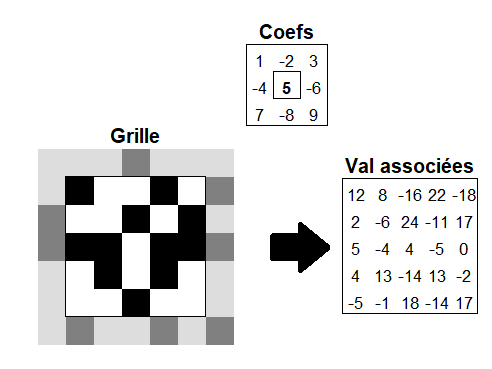
\includegraphics[scale=0.7]{images/imgAlgoNeural/IllustrationArbitraire.png}
        \caption{Illustration du fonctionnement avec des valeurs arbitraires}
\end{figure}
 
 \par \textbf{\textit{Totalement}} par coïncidence, la règle et les coefficients donnés en exemple sont ceux de Conway's Game Of Life : si une cellule est "morte" (vaut 0), alors la valeur x donné à la règle vaut entre 0 et 8, la cellule ne sera "vivante" (vaut 1) à la prochaine étape que si x vaut 3 donc si elle possède exactement 3 cellules voisines vivantes ; tandis que si elle est vivante, x vaut entre 9 et 17, elle ne sera vivante à la prochaine étape si x vaut 11 ou 12, donc si elle possède 2 ou 3 cellules voisines vivantes. A noter que si une cellule se trouve sur un des bords de la grille, les cellules situé sur le bord opposé de la grille peuvent être considéré comme parmi ses voisines ; ainsi toutes les cellules ont toujours 8 voisines.


\begin{figure}[H]
        \center
        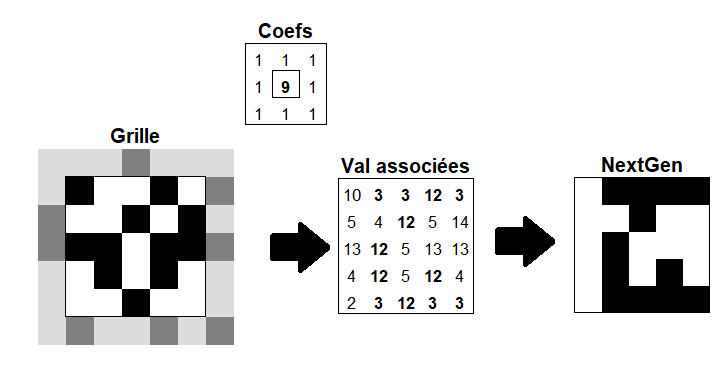
\includegraphics[scale=0.6]{images/imgAlgoNeural/IllustrationGOL.png}
        \caption{Illustration du fonctionnement avec le jeu de la vie}
\end{figure}
 
\par Ces règles peuvent être plus que de simples égalités, et vont souvent renvoyer une valeur entre 0 et 1, plutôt que seulement 0 et 1. Ainsi, avec une combinaison de règle et coefficients minutieuse, il est possible d'observer différents comportements d'algorithmes cellulaires neuraux.

\subsection{Implémentation}

\par \textit{Veuillez noter que, pour une partie des classes utilisées dans les algorithmes cellulaires neuraux et des voisinages de margolus, le nom de celles ci commence par "GOL", ce qui signifie "Game Of Life", et que c'est parfois un abus de langage car le projet porte sur le jeu de la vie, mais ce n'est pas pour autant que toutes les classes sont en rapport au jeu de la vie en tant que tel.}

\par Pour l'implémentation des algorithmes neuraux dans notre projet, on utilise une classe \textit{Grille}, qui est un tableau de taille par taille cellules, taille étant une constante donné à l'initialisation de la Grille, et chaque cellule étant un Float . \textit{Grille} implémente l'interface \textit{Univers}, qui est commun au principe de grilles et de quadtree. \textit{Grille} possède plusieurs méthodes, dont les principales sont \textit{getValAt}, \textit{setValAt}, et \textit{Afficher}. \textit{getValAt} retourne la valeur contenu dans la cellule dont on donne les coordonnées, \textit{setValAt} permet de remplacer les valeur dans une cellule dont on donne les coordonnées par une nouvelle valeur donnée, et \textit{Afficher} permet d'afficher la grille dans l'interface selon plusieurs arguments.

\par Cette \textit{Grille} est utilisé pour les algorithmes neuraux, via la classe \textit{GOLGrilleLifeLike}. Cette classe hérite de \textit{GOLGrille}, qui elle même hérite de la classe abstraite \textit{GOL}, qui sont 2 classes qui mettent les bases pour le fonctionnement des algorithmes neuraux, des voisinages de Margolus, mais aussi de Hashlife cependant uniquement pour la classe \textit{GOL}.

\par \textit{GOLGrilleLifeLike} a besoin de la taille, d'une règle, d'un mode, d'un randType, et optionnellement d'une couleur (qui n'est donc pas importante pour le fonctionnement de la classe) afin de faire fonctionner ses méthodes les plus importantes. Voici l'utilisation de ces variables, ainsi que les méthodes importantes :
\begin{itemize}
    \item La taille est la largeur et la hauteur de la grille, et cette dernière est créée dans le constructeur.
    \item La règle est utilisé pour créer une instance de \textit{DecodeGrilleLifeLike}, qui est une classe utilisé pour transformer la règle, qui est un String, en un tableau de coefficients, si la règle est conforme aux attentes pour une règle d'algorithmes neuraux : 9 nombres séparé par des "/", chaque nombre correspondant au coefficient pour l'une des positions de cellules pour la convolution.
    \item Le randType détermine, lorsqu'on tente de remplir la grille de valeur aléatoire via la méthode \textit{randomizeUnivers}, si la grille est rempli de 0 et de 1, ou si elle est rempli de valeurs flottantes entre 0 et 1, ou si la grille ne peut pas être rempli aléatoirement, en appelant respectivement les méthodes \textit{randomizeUniversBin}, \textit{randomizeUniversFloat}, ou aucun appel de méthodes. Le randType est utile car certains algorithmes fonctionnent sur des grilles où les valeurs ne peuvent avoir que 2 états, comme le jeu de la vie qui a des cellules qui ne peuvent être que "vivantes" ou "mortes", et d'autres qui sont adapté à avoir une situation initiale et ne pas être modifié via une grille aléatoire.
    \item Le mode est une valeur qui permet à la méthode \textit{tick} de savoir quel est l'algorithme neural qui dois être utilisé. La méthode \textit{tick} crée une nouvelle grille vide, et la rempli des valeurs de l'étape suivante de l'algorithme à l'aide du mode et du tableau de coefficient créé par l'instance de \textit{DecodeGrilleLifeLike}, et la renvoie.
    \item La couleur est un tableau de 3 valeurs entre 0 et 1, qui permettent d'accentuer une couleur lors de l'affichage de la grille (chaque valeur accentue respectivement le rouge, le vert, et le bleu). La plupart du temps, les valeurs sont de 0, ce qui permet un affichage en noir pour les cellules valant 1, blanc pour celles valant 0, et en teintes de gris pour les valeurs entre 0 et 1.
\end{itemize}

\par Ainsi, le fonctionnement des Algorithmes cellulaires neuraux est assuré par les méthodes décrites si dessus. Il est ensuite possible d'appeler depuis une classe qui coordonne toutes les autres classes une méthode \textit{update}, qui va changer la grille contenue dans l'instance de \textit{GOLGrilleLifeLike} en son étape suivante selon la méthode \textit{tick}, donc selon l'algorithme, et cette grille peut être affichée grâce à sa méthode \textit{Afficher}.

\begin{figure}[H]
        \center
        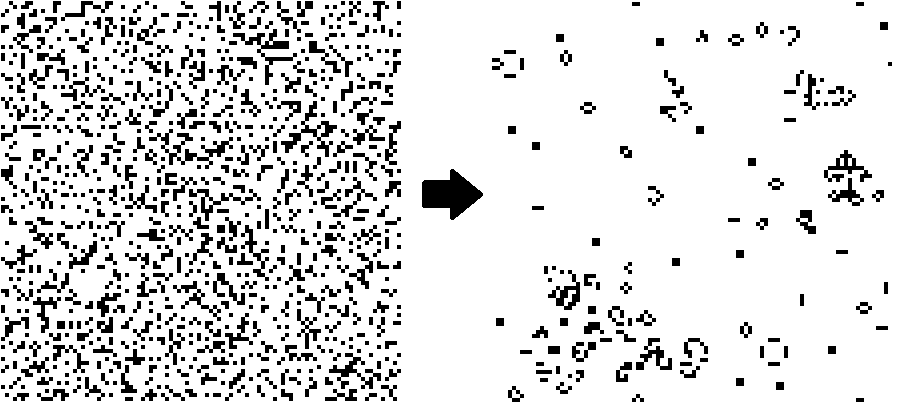
\includegraphics[scale=0.5]{images/imgAlgoNeural/GOLAvantApres.png}
        \caption{Jeu de la vie : début aléatoire $\rightarrow$ 1000 générations plus tard}
\end{figure}

\begin{figure}[H]
        \center
        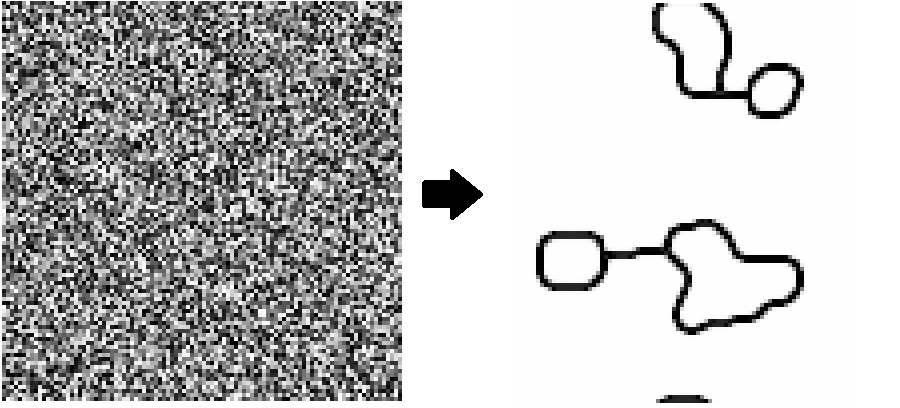
\includegraphics[scale=0.5]{images/imgAlgoNeural/PathwaysAvantApres.png}
        \caption{Algorithme Pathways : début aléatoire $\rightarrow$ 1000 générations plus tard}
\end{figure}
\section{Voisinages de Margolus}

\par Le voisinage de Margolus est une méthode de voisinage différente du voisinage de Moore, ce qui permet de faire des automates cellulaires différent des algorithmes cellulaires neuraux. Tout comme ce dernier, il existe énormément de règles pour les voisinages de Margolus pouvant être intéressante, par exemple celles de \href{https://dmishin.github.io/js-revca/}{ce site}, dont on a implémenté les règles données.

\subsection{Fonctionnement}

\par Le voisinage de Margolus sont utilisés sur des grilles de taille finie de cases, ou cellules, qui possèdent une valeur qui est soit 0, soit 1, et consistent à regrouper les cellules en groupe de 2x2 cellules, auquel on associe une valeur selon si les cellules du groupe valent 0 ou 1, et cette valeur accompagné par la règle de l'automate cellulaire, remplace le groupe de 2x2 cellules par un autre.

\par Les groupes de 2x2 cellules sont déterminé par leur position, mais aussi par le nombre de générations déjà effectués : à la première génération, on crée les groupe en partant de chaque duos de coordonnées paires : un groupe qui commence en (0,0) (qui englobe donc les cases (0,0), (0,1), (1,0) et (1,1) ), en (0,2), en (2,0) etc... tandis qu'à la seconde génération, On crée les groupes en partant de chaque duos de coordonnées impaires ; on alterne ensuite entre chaque génération. A noter que dans le cas de notre implémentation, des cellules situé sur bord de la grille peuvent créer un groupe avec des cellules situé sur le bord opposé de la grille ; Ainsi si la grille a une taille paire, toutes les cellules feront partie d'un groupe à chaque génération.

\par La façon dont les valeurs sont calculées est similaire à du binaire : dans chaque groupe de 2x2 cellules, on associe la valeur de la cellule en haut à gauche avec le premier bit en partant de la droite, la cellule en haut à droite avec le second, celle en bas à gauche avec le troisième, et celle en bas à droite le quatrième. Ainsi, un groupe dont les 2 cellules du haut valent 1, et celle en dessous 0, la valeur associé à ce groupe est 0011 en binaire, soit 3 en base 10 ; un groupe sont la seule cellule qui vaut 1 est en bas a droite à comme valeur associé 1000 en binaire, soit 8 en base 10. Un groupe peut donc avoir une valeur associé entre 0000 et 1111, c'est à dire entre 0 et 15.


Image de grille à un moment pair ou impair + val des groupes


\par Le format de règle pour un voisinage de Margolus est une façon d'associer chaque groupe possible avec un autre, qui le remplacera lors de la prochaine génération. Le plus simple est d'avoir une liste de 16 valeurs, chacune entre 0 et 15, généralement toutes unique (mais cela n'est pas obligatoire). 

\par Ainsi, chaque groupe de cellules est converti en une valeur décimale, qui est associé à une autre valeur via la règle, est qui de nouveau converti en un groupe de cellules, qui remplacera le groupe de départ lors de la prochaine génération.

\subsection{Implémentation}

\par Similairement aux algorithmes cellulaires neuraux, les voisinages de Margolus se servent de la classe \textit{Grille}, que l'on ne va pas réexpliquer.

\par La classe principale pour les voisinages de Margolus est \textbf{GOLGrilleMargolus}, qui hérite de \textit{GOLGrille}, aussi déjà expliqué dans les algorithmes cellulaires neuraux. Celle classe nécessite une taille, une règle, et optionnellement une couleur. La taille est celle de la grille, et la règle est utilisé pour initialiser une instance de \textit{DecodeGrilleMargolus}.

\par \textit{DecodeGrilleMargolus} fonctionne similairement à \textit{DecodeGrilleLifeLike}, à l'exception que la règle doit être une suite de 16 nombres entiers entre 0 et 15 séparés par des "/", et si la règle est correcte, alors ils sont stocké dans l'ordre dans un tableau, et pour une valeur "x" représentant un groupe de cellule donnée, tab[x] sera la valeur correspondant au groupe de cellule de la génération suivante.

\par \textbf{GOLGrilleMargolus} possèdes aussi des méthodes similaire avec son homologue des algorithmes cellulaires neuraux, \textbf{GOLGrilleLifeLike}, excepté la méthode \textit{tick} : cette méthode crée tous les groupes de 2x2 cellules nécessaires, en prenant en compte si on est sur une génération paire ou impaire afin de décaler ou non la création des groupes, récupère la valeur associé à ce groupe, et crée un nouveau groupe de cellules qui est placé dans une nouvelle instance de \textit{Grille}, qui sera renvoyé à la fin de la méthode.

\begin{figure}[H]
        \center
        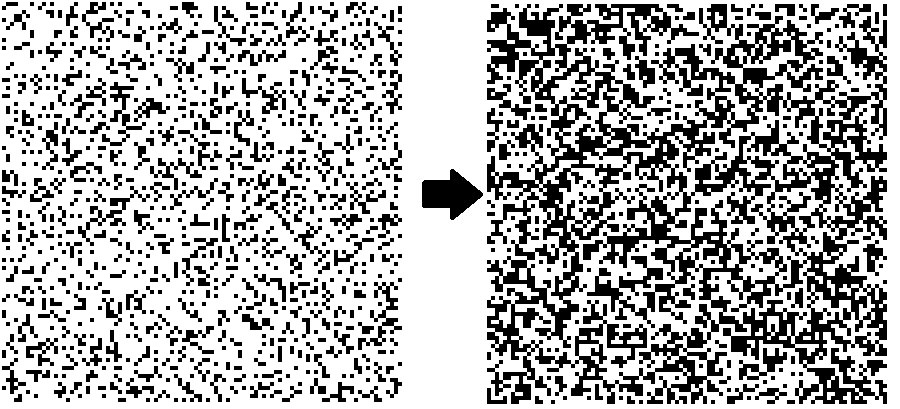
\includegraphics[scale=0.5]{images/imgMargolus/TronAvantApres.png}
        \caption{Algorithme Tron : début aléatoire $\rightarrow$ 1000 générations plus tard}
\end{figure}

\begin{figure}[H]
        \center
        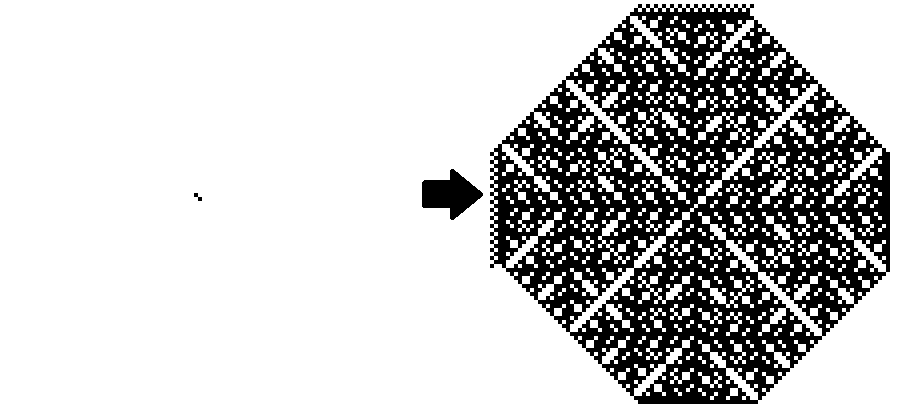
\includegraphics[scale=0.5]{images/imgMargolus/ToothpickAvantApres.png}
        \caption{Algorithme Toothpick : début prédéfini $\rightarrow$ quelques dizaines de générations plus tard}
\end{figure}
\section{Hashlife}
\subsection{un peu d'histoire}
\begin{figure}[htp]
        \center
        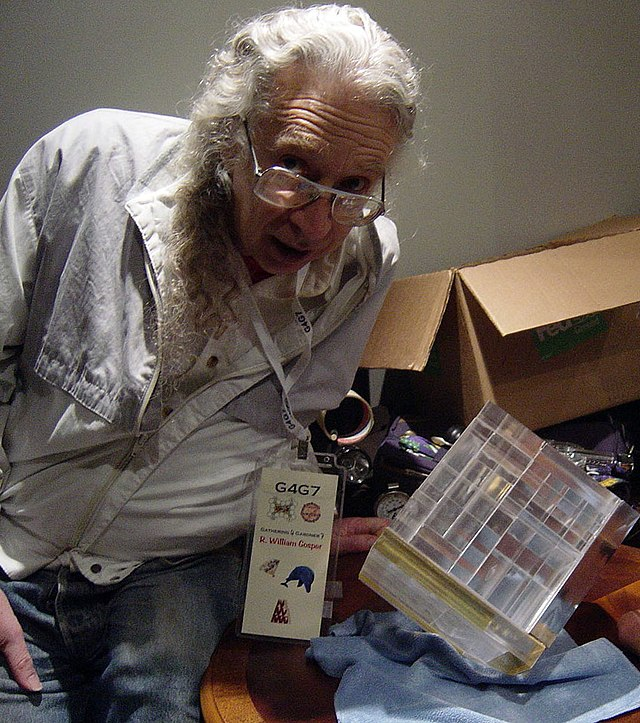
\includegraphics[scale=0.2]{images/imgHashlife/Bill_Gosper_2006.jpg}
        \caption{William (aussi appelé Bill) Gosper l'inventeur de Hashlife}
\end{figure}

Hashlife fut initialement développé en 1984 par le mathématicien William Gosper qui avait pour but d'optimiser la résolution de formes Régulières dans les automates cellulaires, notamment le jeu de la vie de John Conway. A l'époque les mathématiciens et les informaticiens essayaient de développer leur propre algorithme pour optimiser le jeu de la vie. Parmi les méthodes d'optimisations communes, on trouve par exemple l'utilisation complète des registres afin d'économiser de l'espace. Il est aussi possible de reconnaître les oscillateurs et de les pré-calculer pour ne pas avoir à les prendre en compte dans le calcul complet. Cependant, ces optimisations devenaient lourdes et fournissaient des résultats moins intéressants.

En essayant de simplifier les choses, William Gosper crée alors l'algorithme Hashlife. Il publie donc \textit{"Exploiting Regularities in Large Cellular Spaces"}, un article détaillant son algorithme.

Toutefois, étant donné la complexité de l'algorithme, aucune implémentation ne sera créée directement après la publication de cet article, ce qui le cachera initialement du grand public et retardera son implémentation. Hashlife devient alors la source de rumeurs pendant les années 80 lorsque Rudy Rucker déclara avoir été témoin de simulations impressionnantes du jeu de la
vie, lors d'une visite chez William Gosper. 

Épaté, il dira bien plus tard : 

\textit{"Gosper showed me some incredible game of life simulations that were based on a weird speed-up algorithm of his, called 'Hashlife'. I remember him sharing the source code for the trick, but for me that was strictly a case of the Mathematician Godfather: He makes you an offer you can't understand"}

Plusieurs années plus tard, en 2005, sort GOLLY l'une des premières implémentations de Hashlife, ainsi que de Quicklife. Cette implémentation deviendra rapidement la référence dans le monde du jeu de la vie. Elle permet en effet de simuler des univers du jeu de la vie absolument gigantesques - grâce à des optimisations de mémoire - à des vitesses hallucinantes. En effet, GOLLY utilise Quicklife dans les cas ou Hashlife est trop lent. L'intérêt du public pour ce logiciel est sans précédent et permet de populariser le jeu de la vie.

\subsection{Aperçu}
Comme dit précédemment, Hashlife est un algorithme utilisé pour optimiser les formes de vie régulières dans le jeu de la vie. Cependant, grâce à l'augmentation de la taille de la mémoire de nos ordinateurs, l'algorithme est plus généraliste. Il peut optimiser plus de conditions, et il n'est donc plus très pertinent de développer une solution hybride pour un projet simple.

Mais qu'optimise Hashlife?

Dans le jeu de la vie classique, il existe deux grandes limitations :
\begin{itemize}
\item{La vitesse}
\item{La taille}
\end{itemize}
William Gosper décide donc d'orienter son attention vers ces limitations.

Pour régler le problème de la taille de la simulation, on change de structure de données. C'est à dire que l'on utilise un quadtree sur lequel on effectue une génération du jeu de la vie sans décompresser le quadtree.

Pour optimiser la vitesse, on mémoize les nodes déjà utilisées afin de les réutiliser quand on en a besoin.

Pour aller plus loin, on utilise ce que Gosper appelle la "superspeed", cette partie de l'algorithme qui est responsable du gain de vitesse phénoménal de Hashlife.

\subsection{Compression de l'espace}
\subsubsection{QuadLife}

La base de Hashlife réside dans l'utilisation de quadtrees pour stocker les cellules de notre univers. Un quadtree, aussi appelé "arbre quaternaire" dans le pays des baguettes, est une structure de données arborescente représentée de cette manière : 

\begin{figure}[htp]
        \center
        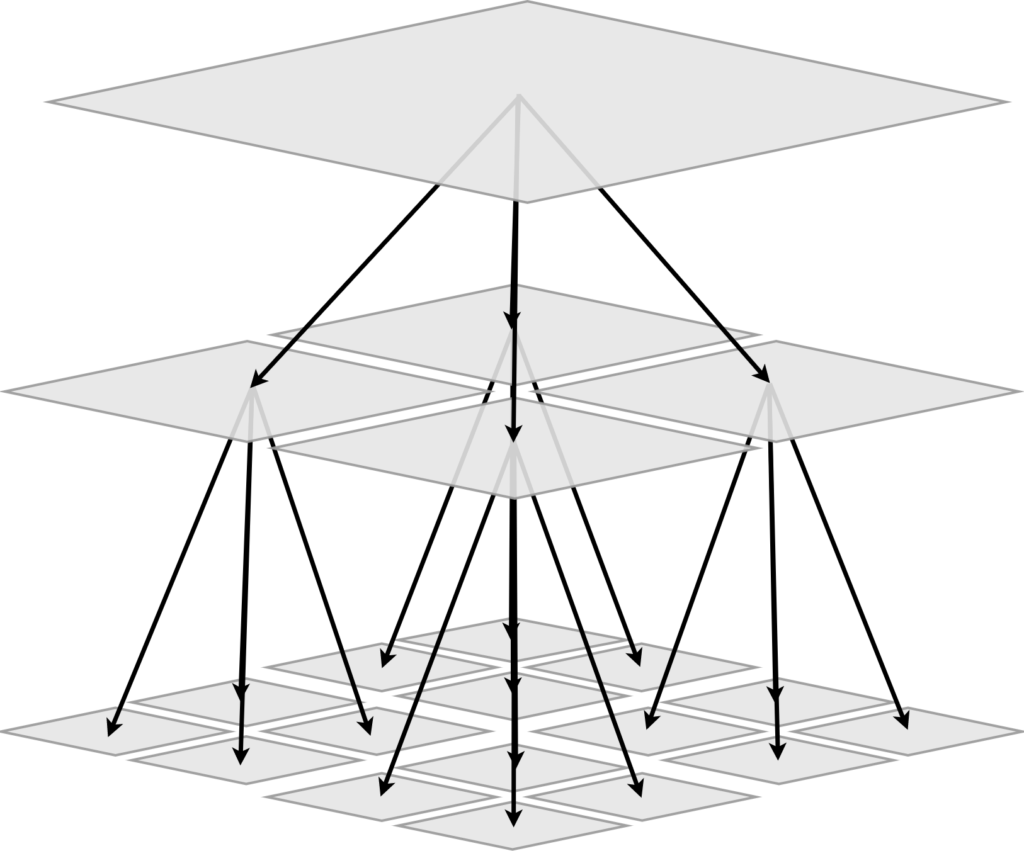
\includegraphics[scale=0.1]{images/imgHashlife/representationquadtree.png}
        \caption{représentation simple d'un quadtree}
\end{figure}

Elle est plus communément utilisée dans la compression de couleurs pour les images, mais cette structure de données a bien d'autres applications, l'une d'entre elle étant évidemment Hashlife!

\begin{figure}[htp]
        \center
        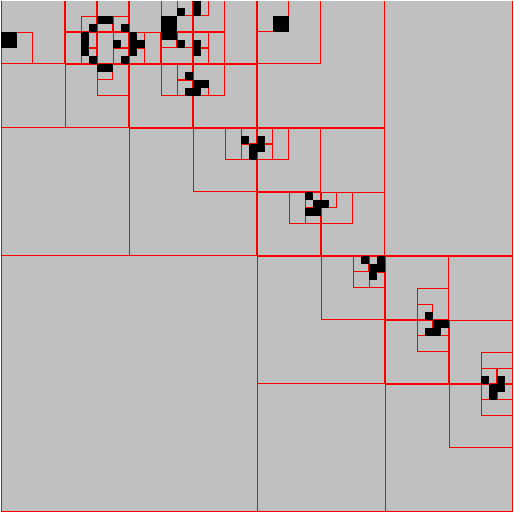
\includegraphics[scale=0.2]{images/imgHashlife/quadLife1.png}
        \caption{utilisation de Quadtree pour stocker un pistolet à Gliders dans notre projet}
\end{figure}

Rajouter des cellules vivantes à un quadtree est en réalité assez simple.
Il faut juste avoir défini au préalable la taille de notre univers (forcément en puissance de 2 car un quadtree ne peut que représenter des puissances de 2) puis utiliser une fonction récursive pour traverser le quadtree jusqu'à atteindre le niveau 0 et mettre la case à la valeur désirée. On peut aussi obtenir la valeur d'une cellule spécifique exactement de la même manière. On peut donc, si on le veut, implémenter le jeu de la vie de cette manière, mais cela serait extrêmement inefficace et empirerait notre problème de vitesse ainsi que de taille car on aurait alors décompressé notre quadtree.

Il nous faut donc une routine qui effectue le jeu de la vie directement sur un quadtree sans rien décompresser. Cette partie est très complexe mais je vais faire de mon mieux pour essayer de simplifier sans perdre des information clés.

On veut faire une fonction dans laquelle on met un Quadtree en argument et la fonction nous renvoie le Quadtree de prochaine génération qu'on peut en déduire.

Premier problème: on ne peut pas déduire la valeur de toutes les cases du quadtree car celles qui sont collées à la bordure ont des voisins impossibles à déduire car externes à la node concernée. Il faudrait prendre la node parent pour trouver les voisins dans les nodes adjacentes, mais il faudrait alors prendre tout le quadtree (car la node parent a aussi des nodes adjacentes) donc ce n'est pas une solution viable.

\begin{figure}[htp]
        \center
        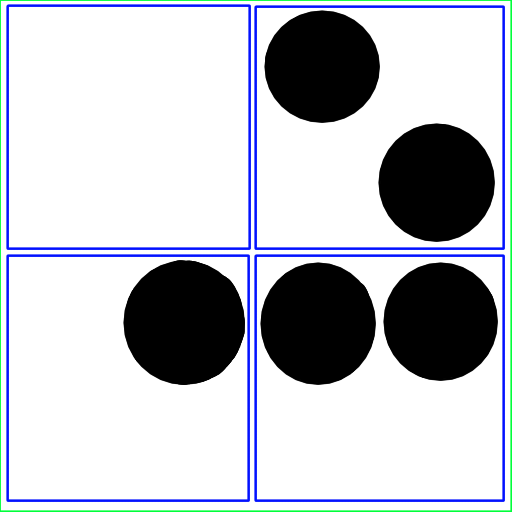
\includegraphics[scale=0.7]{images/imgHashlife/GOLfig1.png}
        \caption{on ne peut pas vérifier tout les voisins des cellules depuis les arbres bleus }
\end{figure}

A la place nous allons nous contenter de renvoyer la node centrale de notre quadtree, c'est ce qui va nous permettre d'éviter de décompresser le quadtree. Essentiellement, nous ne pouvons être sûrs de calculer que les nodes qui ont des voisins dans notre quadtree, nous ne calculons que la node centrale pour laisser les enfants de notre quadtree faire le reste du boulot car la fonction est récursive.

Notre fonction prend donc un quadtree en entrée et renvoie la node centrale de celui-ci à la prochaine génération. Il peut donc sembler correct d'appliquer la fonction sur chaque node mais cela laisserait des "trous" non calculés dans notre quadtree, la fonction ne fonctionne toujours pas complètement...

\begin{figure}[htp]
        \center
        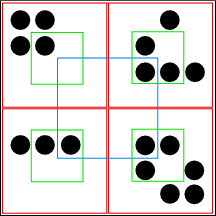
\includegraphics[scale=0.7]{images/imgHashlife/GOLfig2.png}
        \caption{voici pourquoi on ne peut pas simplement renvoyer la node centrale de chaque node. Beaucoup d'espace reste non-calculé et la node centrale initiale n'est pas complètement calculée }
\end{figure}

Notre fonction est cependant "correcte" pour un cas spécifique de notre calcul. Si notre node est juste au-dessus du niveau cellulaire, on peux l'adapter pour calculer directement les quatre cellules qui sont centrales à cet arbre de manière très similaire au jeu de la vie de base. Cette étape est appelé le calcul lent.

On lui crée donc sa propre fonction "calculLent()" qui prend un quadtree de niveau 2 et renvoie un arbre de niveau 1 à la prochaine génération. Notre objectif est à présent d'appeler calcul lent dans toutes les nodes qui arrivent au niveau cellulaire.

\begin{figure}[htp]
        \center
        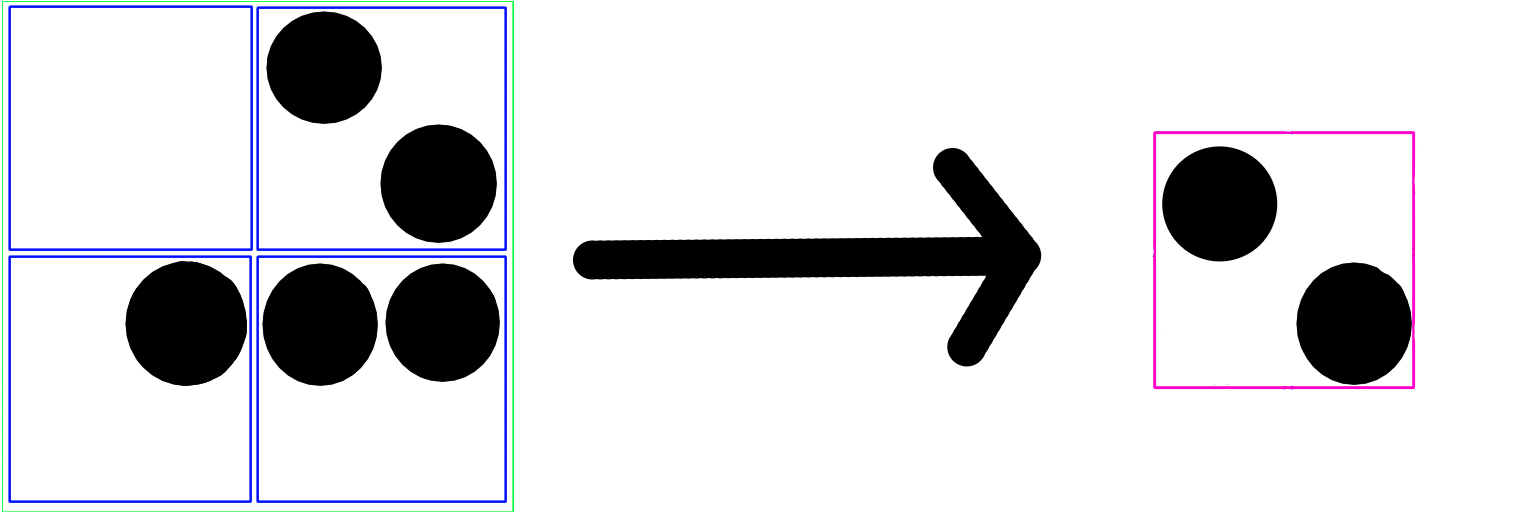
\includegraphics[scale=0.4]{images/imgHashlife/GOLfig3.png}
        \caption{l'arbre violet est le résultat obtenu en appliquant "calculLent()" sur l'arbre vert}
\end{figure}

Pour ce faire, on doit vérifier chaque node non-vide ce qui n'équivaut \textbf{pas} à décompresser le quadtree, vu qu'on ne vérifie pas chaque cellule et qu'on saute les grands espaces vides lorsqu'il y en a.

C'est là que vient la solution de génie: Prenons une node de niveau 3 pour laquelle on veut calculer la prochaine génération de sa node centrale.

Pour ce faire, nous allons générer 9 nodes intermédiaires de niveau 1, puis les rassembler en groupe de 4 pour obtenir des nodes de niveau 2 sur lesquelles on peut utiliser "calculLent()" pour assembler la node centrale de notre node. Rappelez-vous: notre fonction renvoie un arbre deux fois plus petit! Ainsi on a effectué notre prochaine génération sur un arbre de niveau 3. 

\begin{figure}[htp]
        \center
        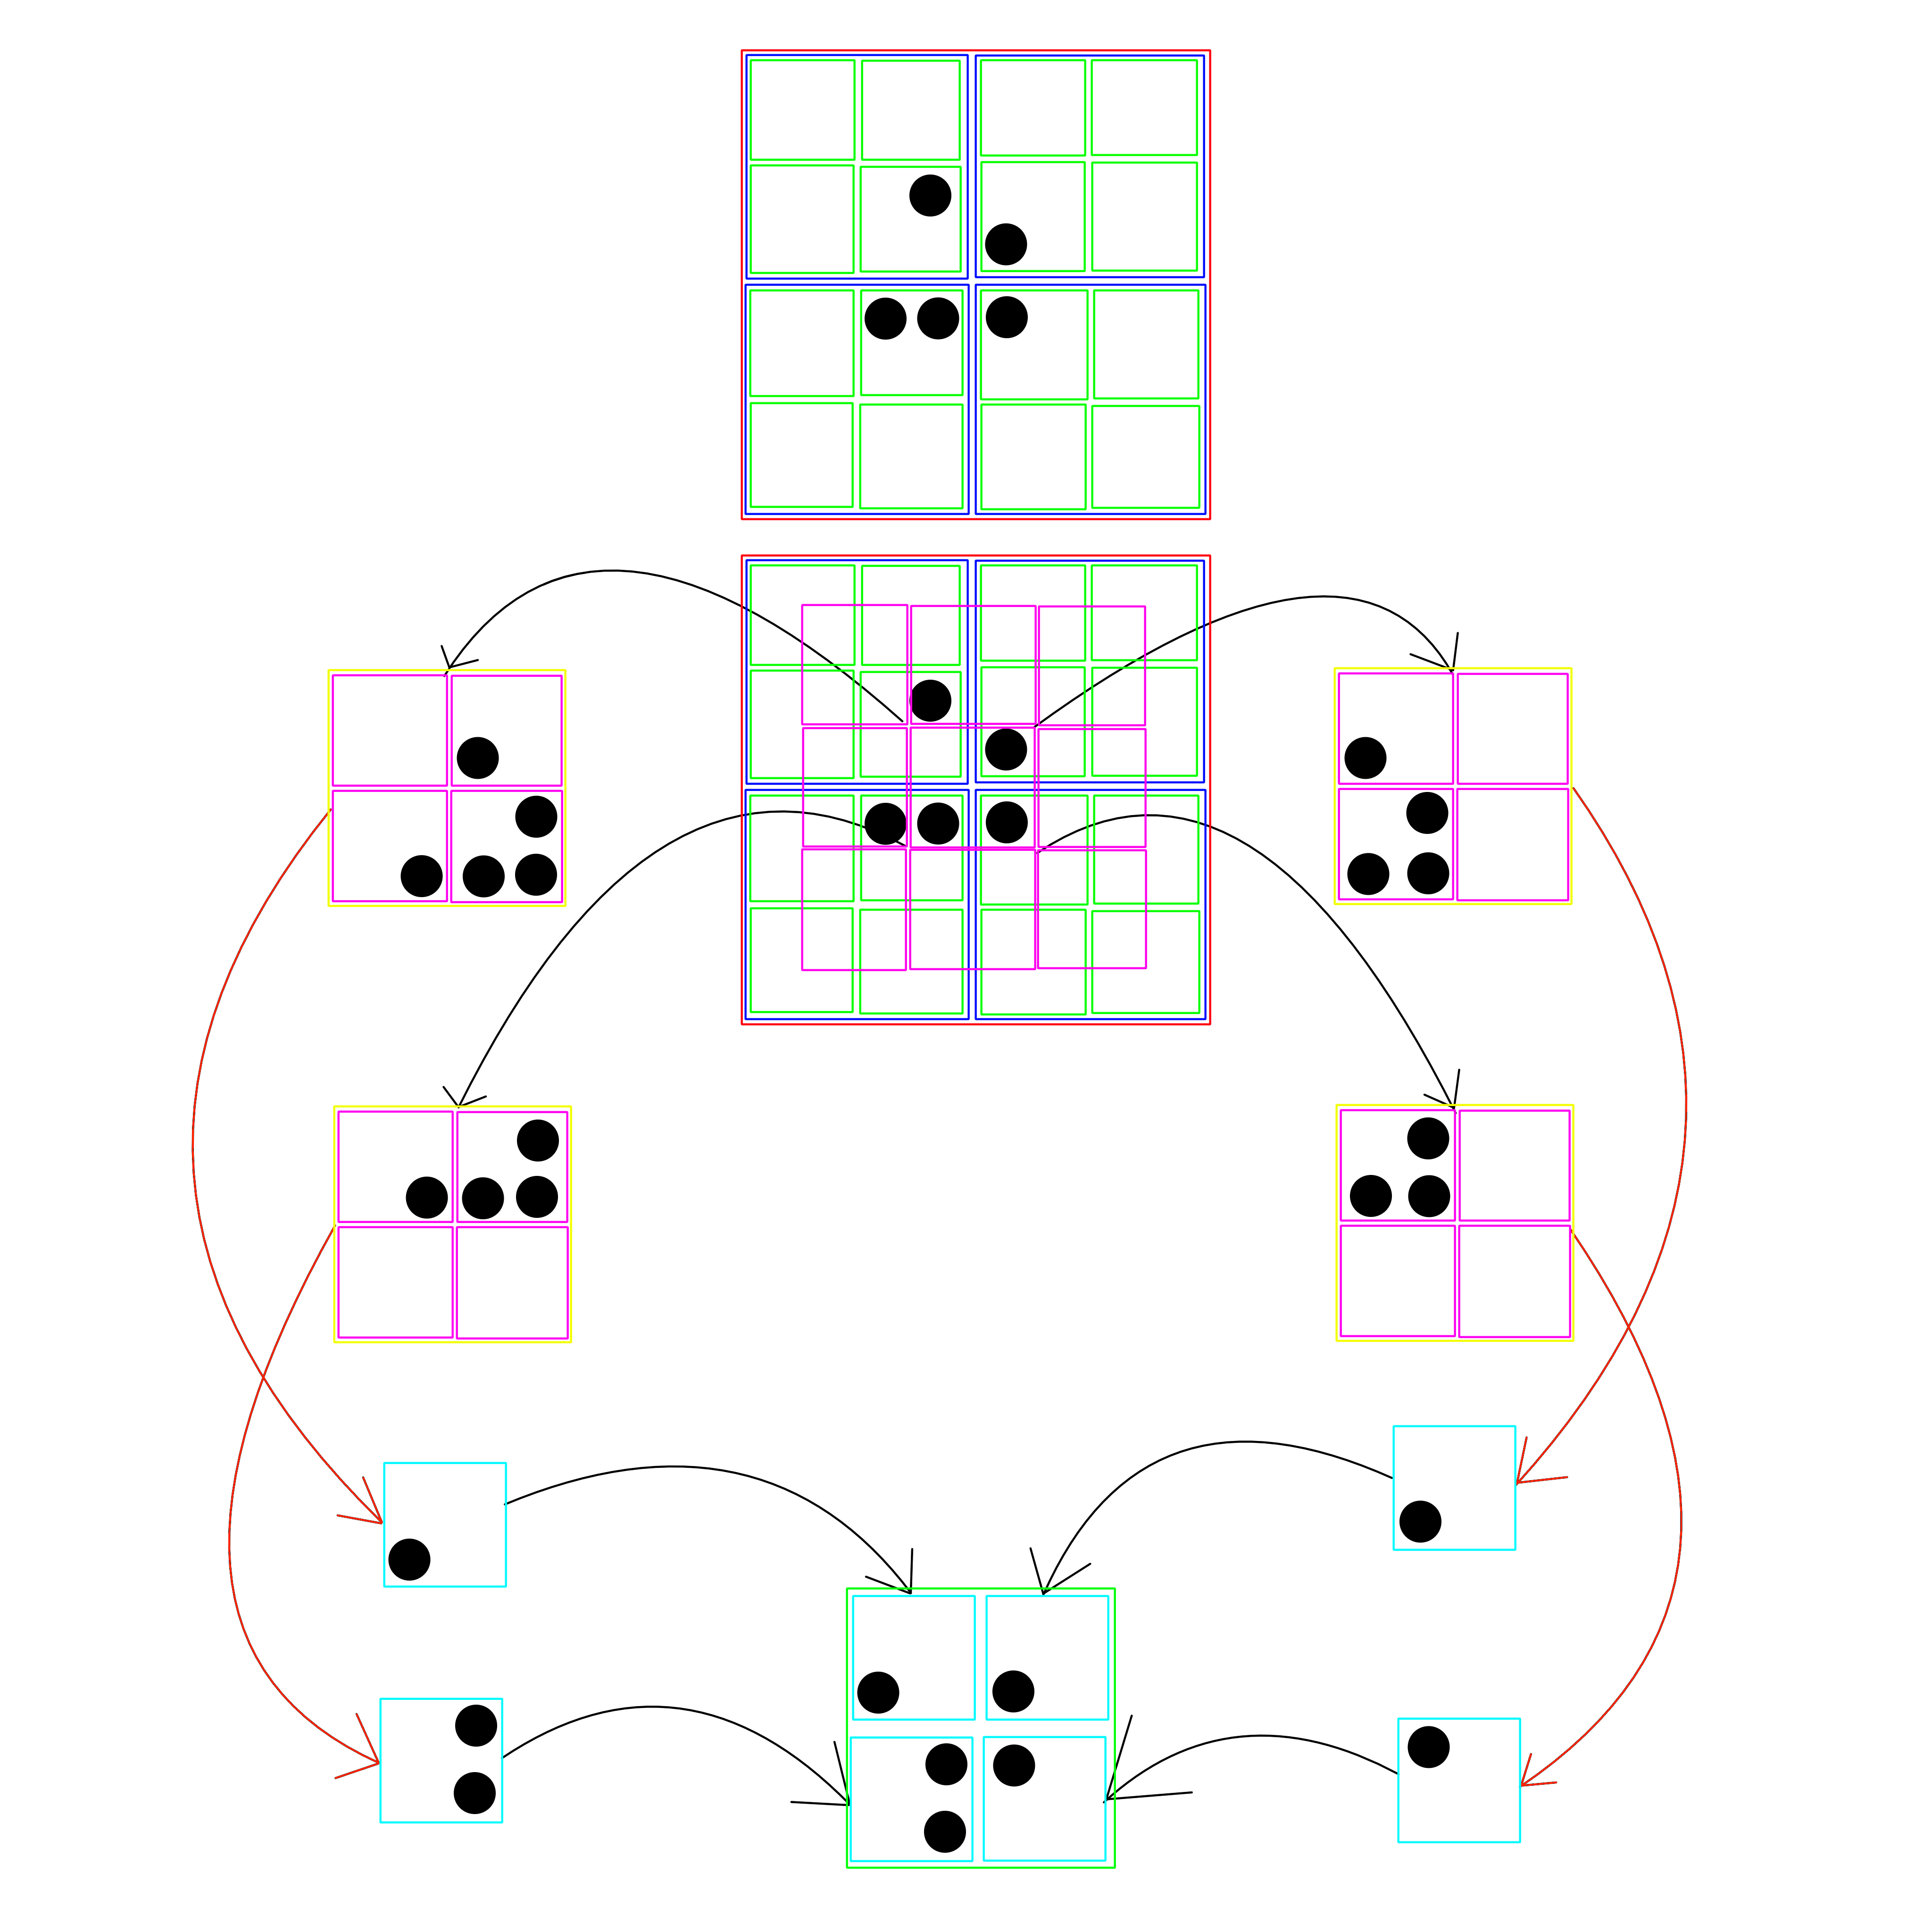
\includegraphics[scale=0.225]{images/imgHashlife/nextGen.png}
        \caption{on groupe les 9 nodes en groupes de 4 sur lesquelles on appelle nextGen (flèches rouges), on assemble le résultat, ce qui nous donne la node centrale une génération en avant de l'arbre initial}
\end{figure}

Chouette! Mais devons-nous répéter l'opération pour chaque node? Heureusement non! Si on met juste une condition pour vérifier si le niveau est égal à 2, alors: si oui, on fait "calculLent()", sinon on fait l'algorithme décrit précédemment. Appelons notre fonction "nextgen()".

\SetKwComment{Comment}{/* }{ */}
\begin{algorithm}
\tiny
\caption{nextgen()}\label{alg:nextgen}
\eIf{level = 2}{
    calculLent()\;
}{
    \Comment{on génère les 9 nodes}
    node1$\gets$ CréerNodeAuxiliaire\_1\;
    node2$\gets$ CréerNodeAuxiliaire\_2\;
    node3$\gets$ CréerNodeAuxiliaire\_3\;
    node4$\gets$ CréerNodeAuxiliaire\_4\;
    node5$\gets$ CréerNodeAuxiliaire\_5\;
    node6$\gets$ CréerNodeAuxiliaire\_6\;
    node7$\gets$ CréerNodeAuxiliaire\_7\;
    node8$\gets$ CréerNodeAuxiliaire\_8\;
    node9$\gets$ CréerNodeAuxiliaire\_9\;
    \Comment{on assemble les 9 nodes en 4 nodes}
    \Comment{on appelle récursivement l'algorithme afin d'obtenir la node centrale}
    \Comment{des 4 nodes à la prochaine génération}
    tmpNode1$\gets$ assembleNode(node1, node2, node4, node5).nextGeneration()\;
    tmpNode2$\gets$ assembleNode(node2, node3, node5, node6).nextGeneration()\;
    tmpNode3$\gets$ assembleNode(node4, node5, node7, node8).nextGeneration()\;
    tmpNode4$\gets$ assembleNode(node5, node6, node8, node9).nextGeneration()\;
    \Comment{on assemble les 4 nodes et on renvoie le résultat}
    resultat$\gets$ assemblerNode( tmpNode1,tmpNode2,tmpNode3,tmpNode4 )\;
}
\end{algorithm}


A ce stade, la partie difficile de cette partie est terminée, mais nous n'avons pas encore fini, en effet si notre algorithme diminue la taille de notre node par 2 à chaque génération, nous n'allons pas pouvoir simuler tout notre quadtree et il rétrécira au fur et à mesure des générations.

La solution est très simple : créer un arbre "bordure" dont la node centrale est l'arbre sur lequel on veut passer à la prochaine génération. Le reste de ses nodes est vide. On appellera cette fonction "extend()".

\begin{figure}[htp]
        \center
        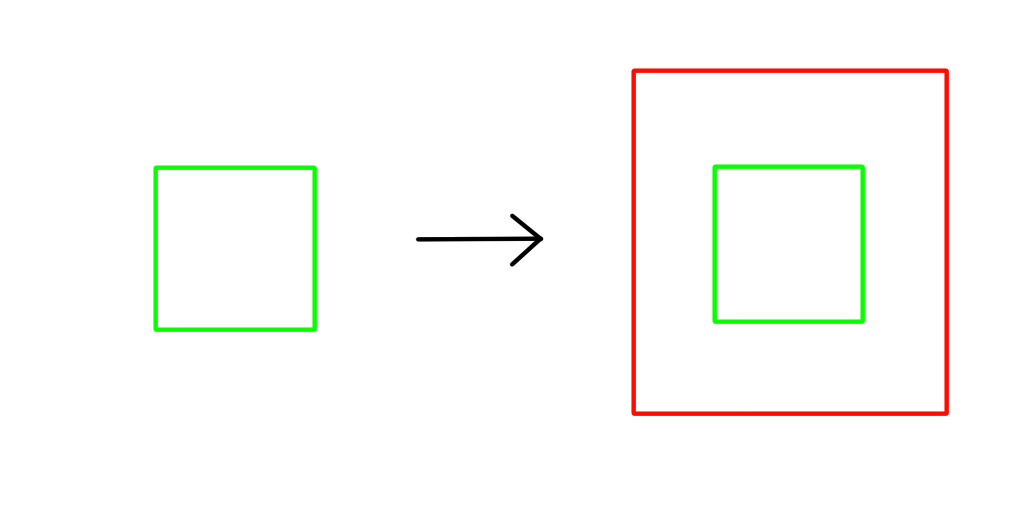
\includegraphics[scale=0.5]{images/imgHashlife/extend.png}
        \caption{l'arbre vert est l'arbre initial, l'arbre rouge est l'arbre bordure, \textit{extend} retourne l'arbre bordure}
\end{figure}

Maintenant il ne nous reste plus qu'à assembler nos fonctions pour créer "fullnextgen()"

Dans un premier temps, on utilise "extend", puis on appelle "nextGen()" et on retourne le résultat. Nous avons maintenant calculé une génération du jeu de la vie dans un quadtree, ce qui n'est pas particulièrement rapide (même plus lent qu'un algorithme classique), de plus l'arbre actuel n'est pas hashable, il faut donc le modifier. Nous n'avons pourtant pas travaillé en vain, notre algorithme permet d'avoir un univers "infini" tant que la population de celui-ci n'est pas trop grosse ce qui résout le premier problème du Jeu de la Vie.

\subsubsection{Canonicalisation du Quadtree}
J'ai mentionné dans la partie précédente que notre arbre n'était pas hashable, en effet, pour obtenir ce statut nous allons devoir procéder à la canonicalisation de notre quadtree.

Qu'est-ce que la canonicalisation d'un quadtree?

En termes simples, "Canonicaliser un arbre" revient à rassembler ses nodes similaires en blocs Canoniques. Ainsi, si une forme est trouvée de multiples fois dans l'arbre, nous ne la stockons qu'une seule fois et nous en passons la référence là ou elle est nécessaire. L'intérêt primordial est de réduire la consommation de mémoire, mais dans le cas de Hashlife cela nous permet d'implémenter la mémoization de manière efficace.

\begin{figure}[H]
        \center
        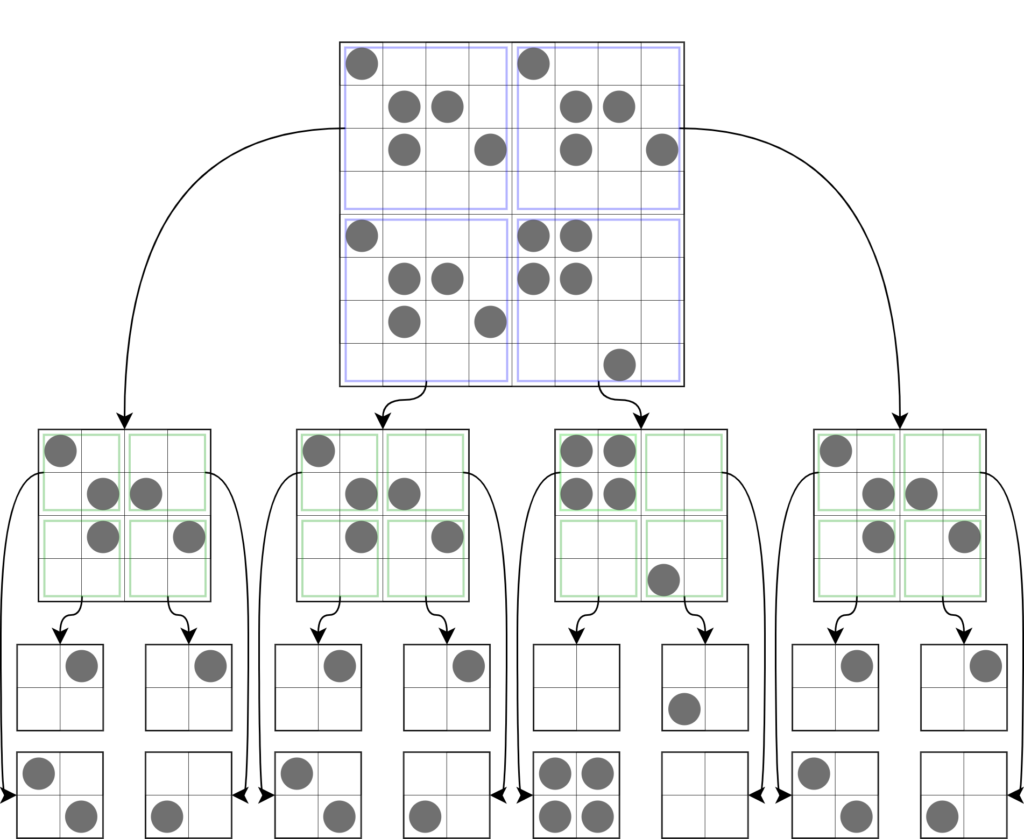
\includegraphics[scale=0.16]{images/imgHashlife/quadtreeNONcanonique.png}
        \caption{voici la représentation de notre arbre actuel, certaines nodes sont identiques et devraient être regroupées!}
\end{figure}

Mais alors, comment allons-nous canoniser notre Quadtree? En théorie c'est en réalité très simple. En effet, il suffit de stocker notre node dans une hashmap avec elle-même comme objet, ainsi quand une node a exactement les mêmes enfants et la même valeur, on peut considérer que les deux objets sont égaux. On peut alors supprimer le nouvel objet et renvoyer la node déjà stockée dans la hashmap. On peut appeler cette fonction "canonicaliser()" ou encore "integre()". Étant donné quelle est moins verbeuse je vais choisir la deuxième option. Finalement, on modifie le constructeur des nodes canoniques afin de les canoniser lors de leur création, on a juste à intégrer la node résultante de la création.

Si on appelle systématiquement le constructeur des nodes canoniques pour créer nos nodes, notre quadtree se canonisera tout seul.

\begin{figure}[H]
        \center
        \includegraphics[scale=0.16]{images/imgHashlife/quadtreecanonique.png}
        \caption{voici la représentation de notre arbre canonisé, les nodes identiques on été regroupées!}
\end{figure}

Même si nous gérons mieux notre mémoire, notre jeu de la vie reste lent. Heureusement, cette étape est la fondation de la partie à suivre qui nous permettra enfin d'aller plus vite qu'une implémentassions classique du jeu de la vie. Il est aussi intéressant de noter que les espaces de forte densité prennent beaucoup moins d'espace que précédemment si ils sont réguliers. Ainsi, nous avons quasiment totalement fait abstraction de la notion d'espace du jeu de la vie.

\subsection{Compression du temps}
\subsubsection{Memoization: Almost-Hashlife}
Maintenant que notre quadtree est canonisé il est trivial d'implémenter la Mémoisation il suffit simplement de rajouter une node appelée next dans notre structure de node, on l'initialisera a null avec le constructeur, cependant on ne prendra pas ce nouveau membre en compte lors de la canonicalisation.
il ne suffit plus que de modifier la fonction "nextGen()" pour vérifier si next est null, si ce n'est pas le cas, on fait le calcul comme précédemment et on initialise next a la valeur du résultat, en revanche si next n'est pas null (et a donc déjà été calculé) on renvoie simplement next.

\begin{algorithm}
\tiny
\caption{nouvelle définition de nextGeneration()}\label{alg:two}
\eIf{next = null}
{
    \Comment{si la node n'est pas calculé on la calcule ici}
    next $\gets$ calculLent()\;
}

\Comment{on renvoie la node précalculée}
resultat $\gets$ next\;
\normalsize
\end{algorithm}

Ainsi on ne refait pas le même calcul deux fois, et après quelques générations énormément de nodes ont été mémoisées, a ce stade l'ordinateur n'effectue quasiment que des lectures dans une hashmap ce qui est très rapide, et ainsi la vitesse d'exécution explose, on est capable de simuler des centaines de génération en une secondes, de plus si le pattern simulé est régulier, il est possible que l'arbre entier soit mémoisé totalement, a ce stade la simulation deviens stable et on n'utilise plus du tout "calculLent()" ce qui va nous permettre de simuler des dizaines de milliers de générations en une seconde, ce qui est vraiment incroyable, mais vu que la simulation n'évolue plus, un peu ennuyant...

On a maintenant un algorithme extrêmement rapide, probablement bien plus rapide que tout autre implémentation du jeu de la vie, même quicklife ne peut pas nous rattraper en nombre de génération par secondes, on pourrait s'arrêter là si on le voulait, la vitesse est suffisante pour simuler des patterns comme le triangle de Sierpinski a des échelles remarquables. Il est a noter que la vitesse est suffisante, nous voulons aller au delà, et c'est ce que va nous permettre Hashlife.
\subsubsection{Superspeed: Hashlife}
Almost-Hashlife nous permet de calculer génération par génération  le jeu de la vie dans un espace quasi-infini, le temps de calcul entre deux génération est le plus petit possible et ne peut être réduit que grâce a des optimisations de bas niveaux comme l'utilisation complète et efficace des registre, du parallélisme SIMD ou du multithreading "simple". Mais d'un point de vue purement algorithmique nous avons atteint le temps de calcul minimal. Mais alors comment accélérer encore plus la simulation? la solution est en réalité plutôt simple : calculer plus de générations pour chaque appel de nextGen(). Pour bien illustrer l'optimisation que nous allons implémenter nous devons revenir a l'implémentation de Quadlife que nous avons abordé précédemment:

Pour passer a la prochaine génération nous générons neufs nodes intermédiaires que nous assemblons pour former quatre nodes sur lesquelles on appelle nextGen() récursivement afin de passer a la prochaine génération Comme montré dans la figure 7.

Pour un arbre de niveau 3 nos 9 nodes temporaires sont de niveau 3-2 = 1, cela ne doit pas changer, cependant, nous allons changer d'approche pour les générer, a la place d'aller chercher  individuellement les 4 nodes nécessaires pour la fabrication de chacune des 9 nodes temporaires individuelles, nous allons prendre des arbres un niveau plus haut ainsi la node temporaire centrale sera la node centrale de l'arbre sur lequel on a appelé nextGen qui est dans notre exemple de niveau 3-1 = 2 les nodes temporaires nw , ne , sw et se sont simplement les enfants correspondants de notre arbre initial, les nodes n, s , w et e sont des mélanges entre les nodes diagonales ex : le bas de nw et le haut de sw combiné donne w.
\begin{figure}[H]
        \center
        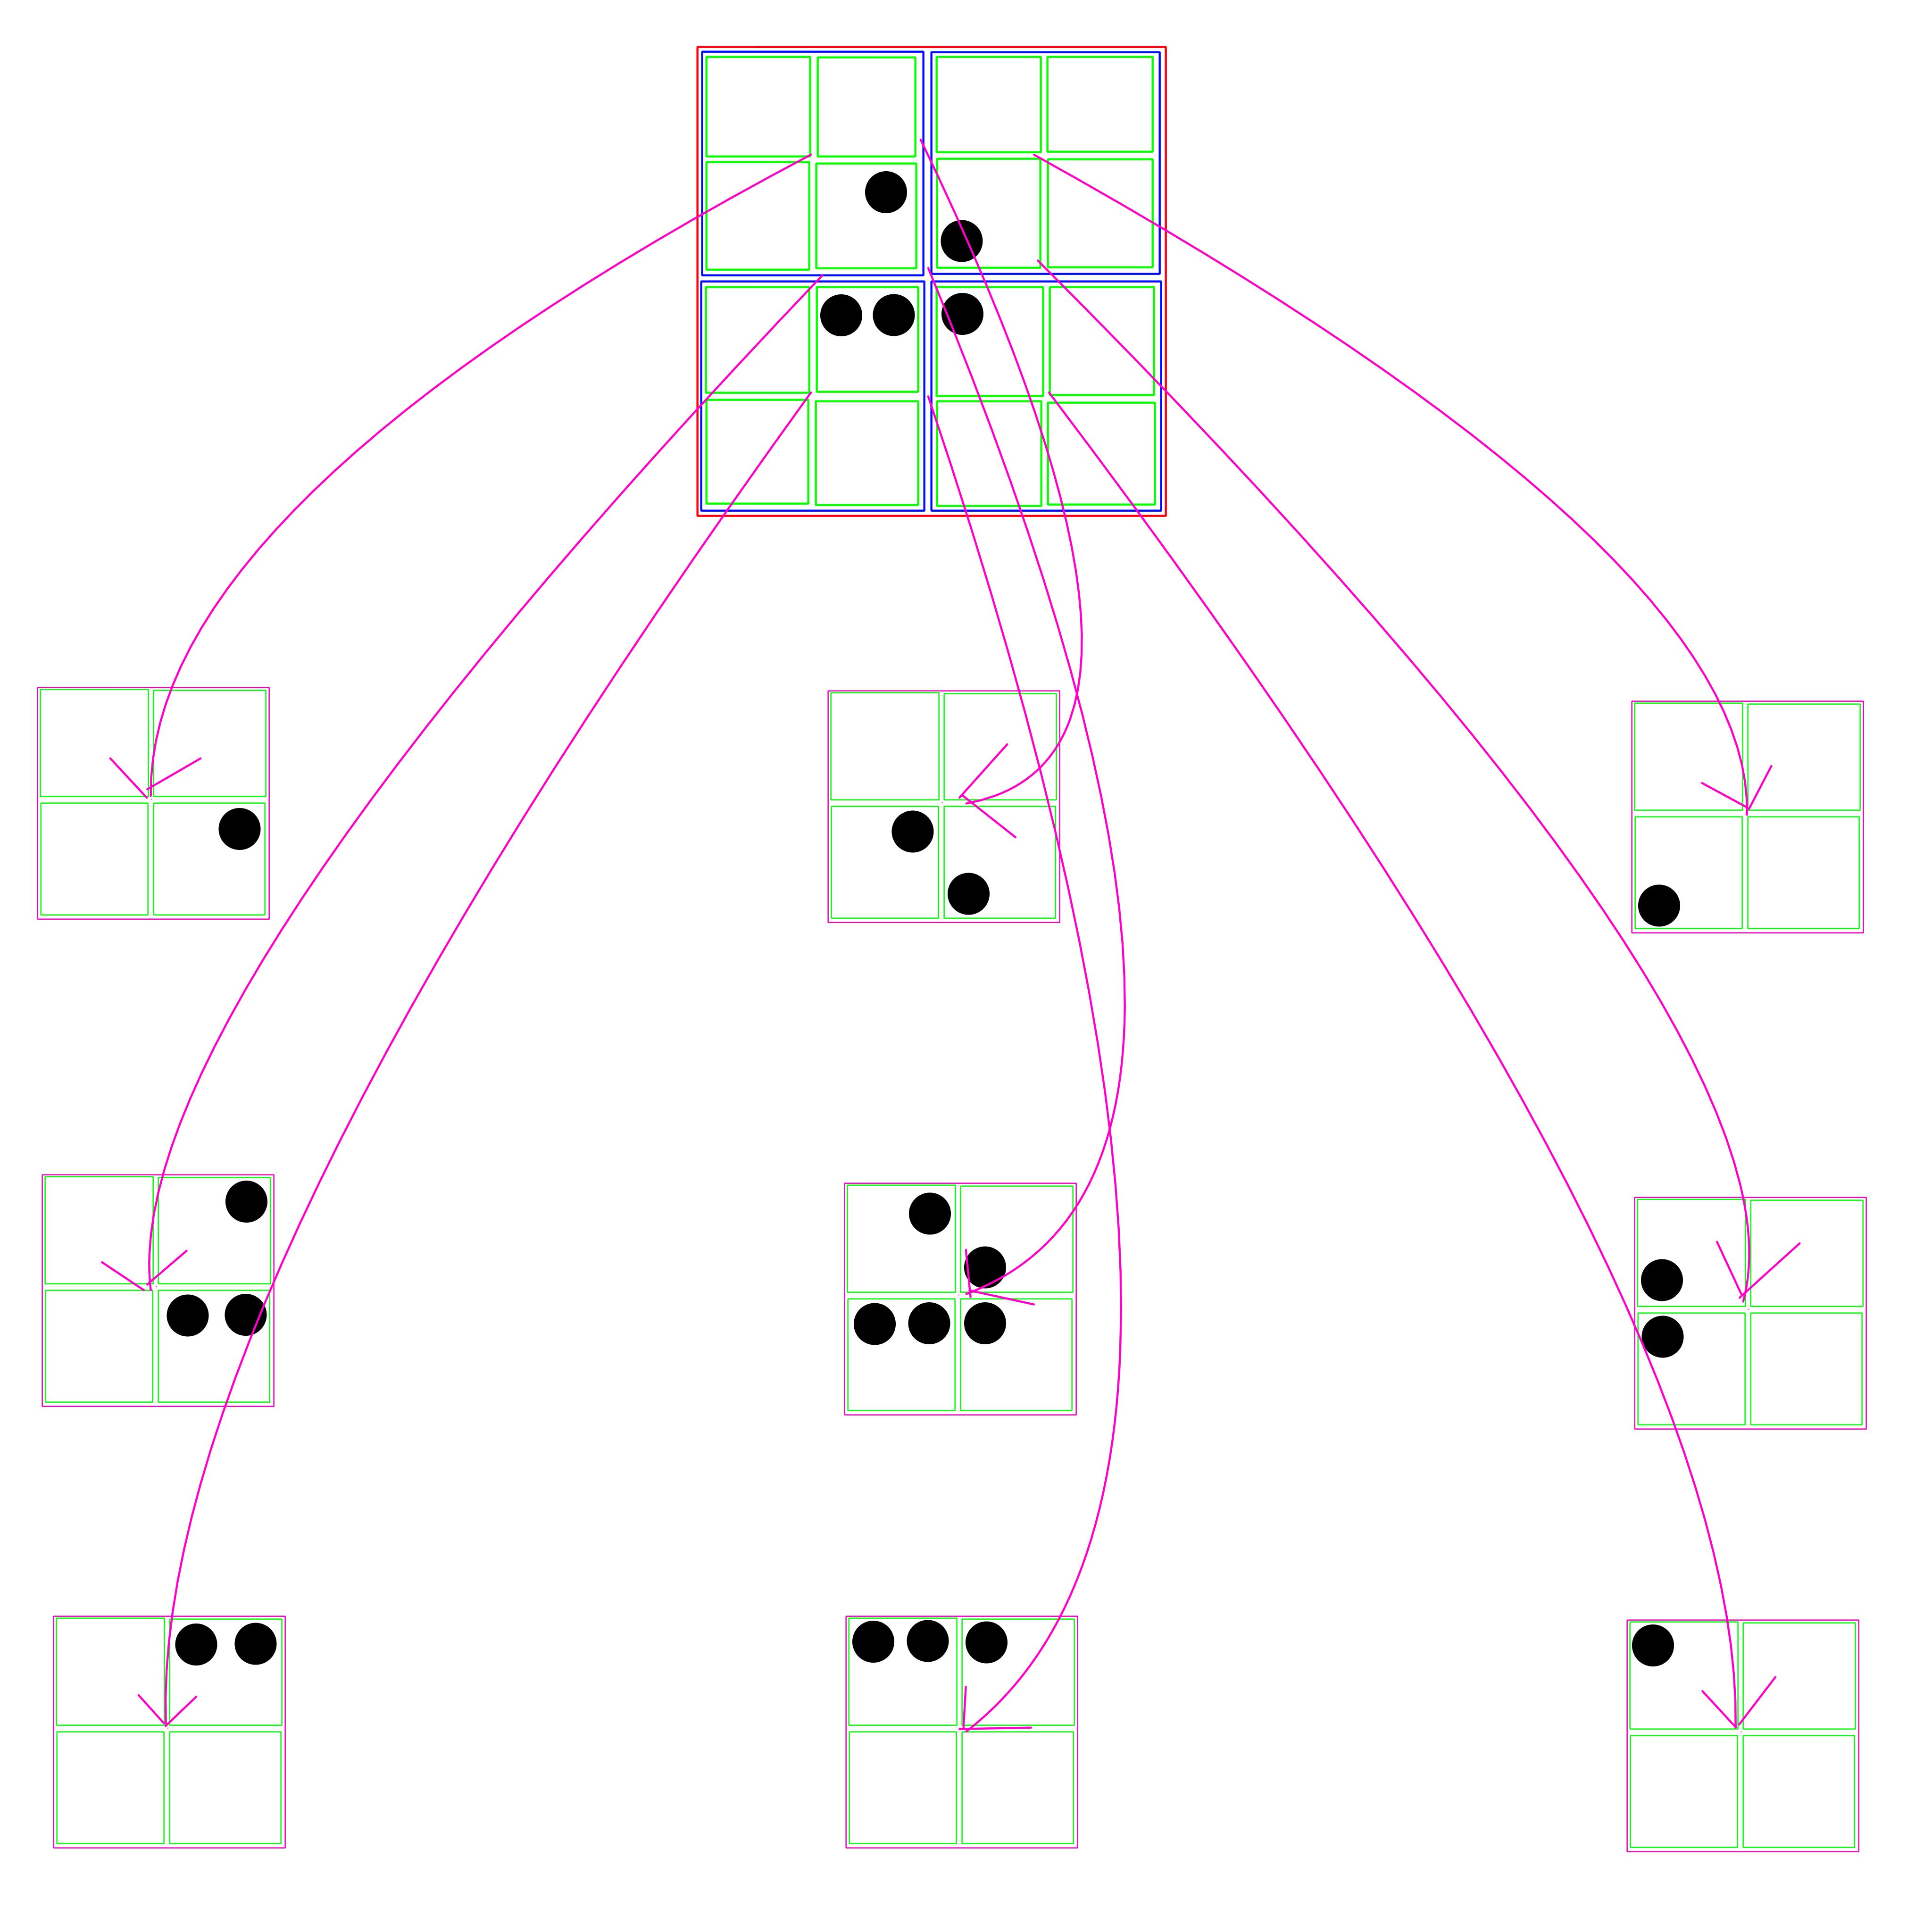
\includegraphics[scale=0.1]{images/imgHashlife/HashlifeStep1.png}
        \caption{Première étape de l'algorithme de Hashlife}
\end{figure}
Ces nouvelles nodes temporaires sont de niveau 2 comme dit précédemment, il faut que nous retrouvons nos nodes de niveau 1, pour les retrouver on pourrait prendre leur node centrale, mais on n'aurais rien fait de très intéressant, a la place nous allons utiliser nextGen pour trouver leur node centrale une génération en avant puis les assembler en nos 4 nodes.
\begin{figure}[H]
        \center
        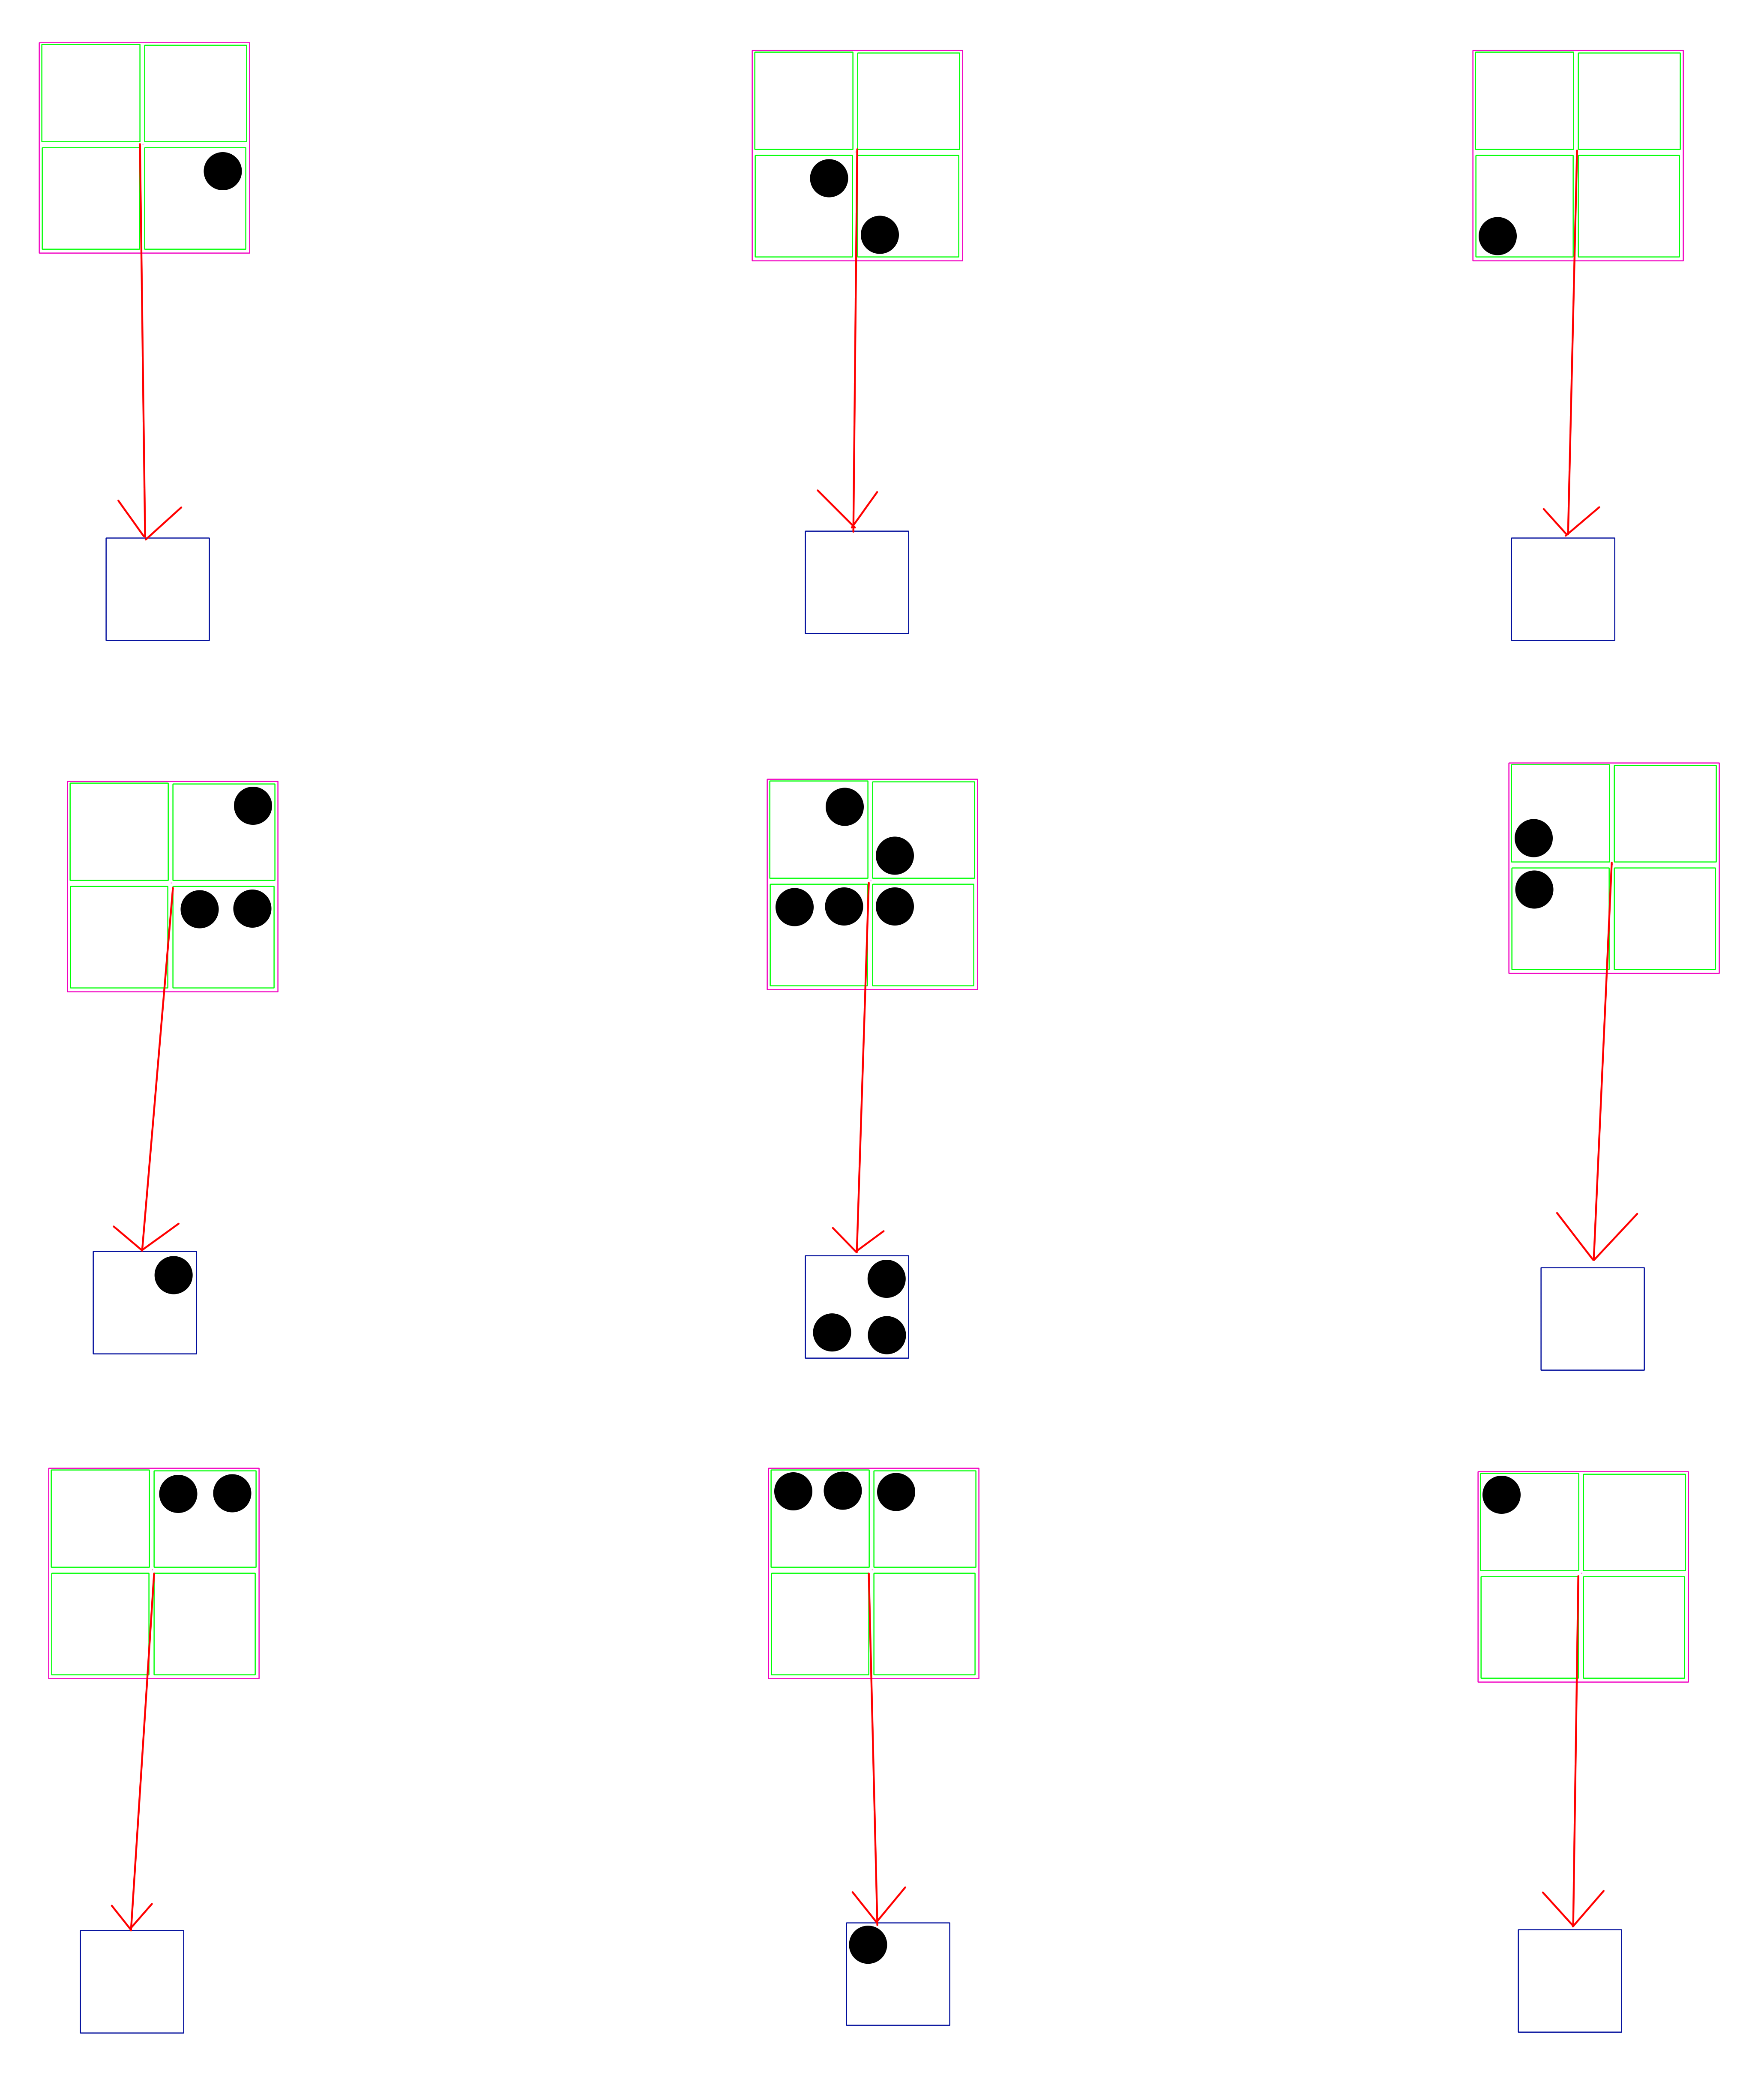
\includegraphics[scale=0.1]{images/imgHashlife/HashlifeStep2.png}
        \caption{Deuxième étape de l'algorithme de Hashlife}
\end{figure}
Nous pouvons alors réutiliser nextGen dessus comme "d'habitude" afin de trouver notre node évoluée cette fois ci non pas d'une génération mais de 2 générations! si on applique l'algorithme sur un niveau plus haut (4) on remarque que l'on ne fait pas 2 mais 4 génération en un seul appel! Et la tendance continue, pour un arbre de niveau 8 on fait 64 générations! Si vous avez l'oeil vous remarquerez que c'est une croissance exponentielle d'écrite par l'équation nbGen = $2^{niveau-2}$.
\begin{figure}[H]
        \center
        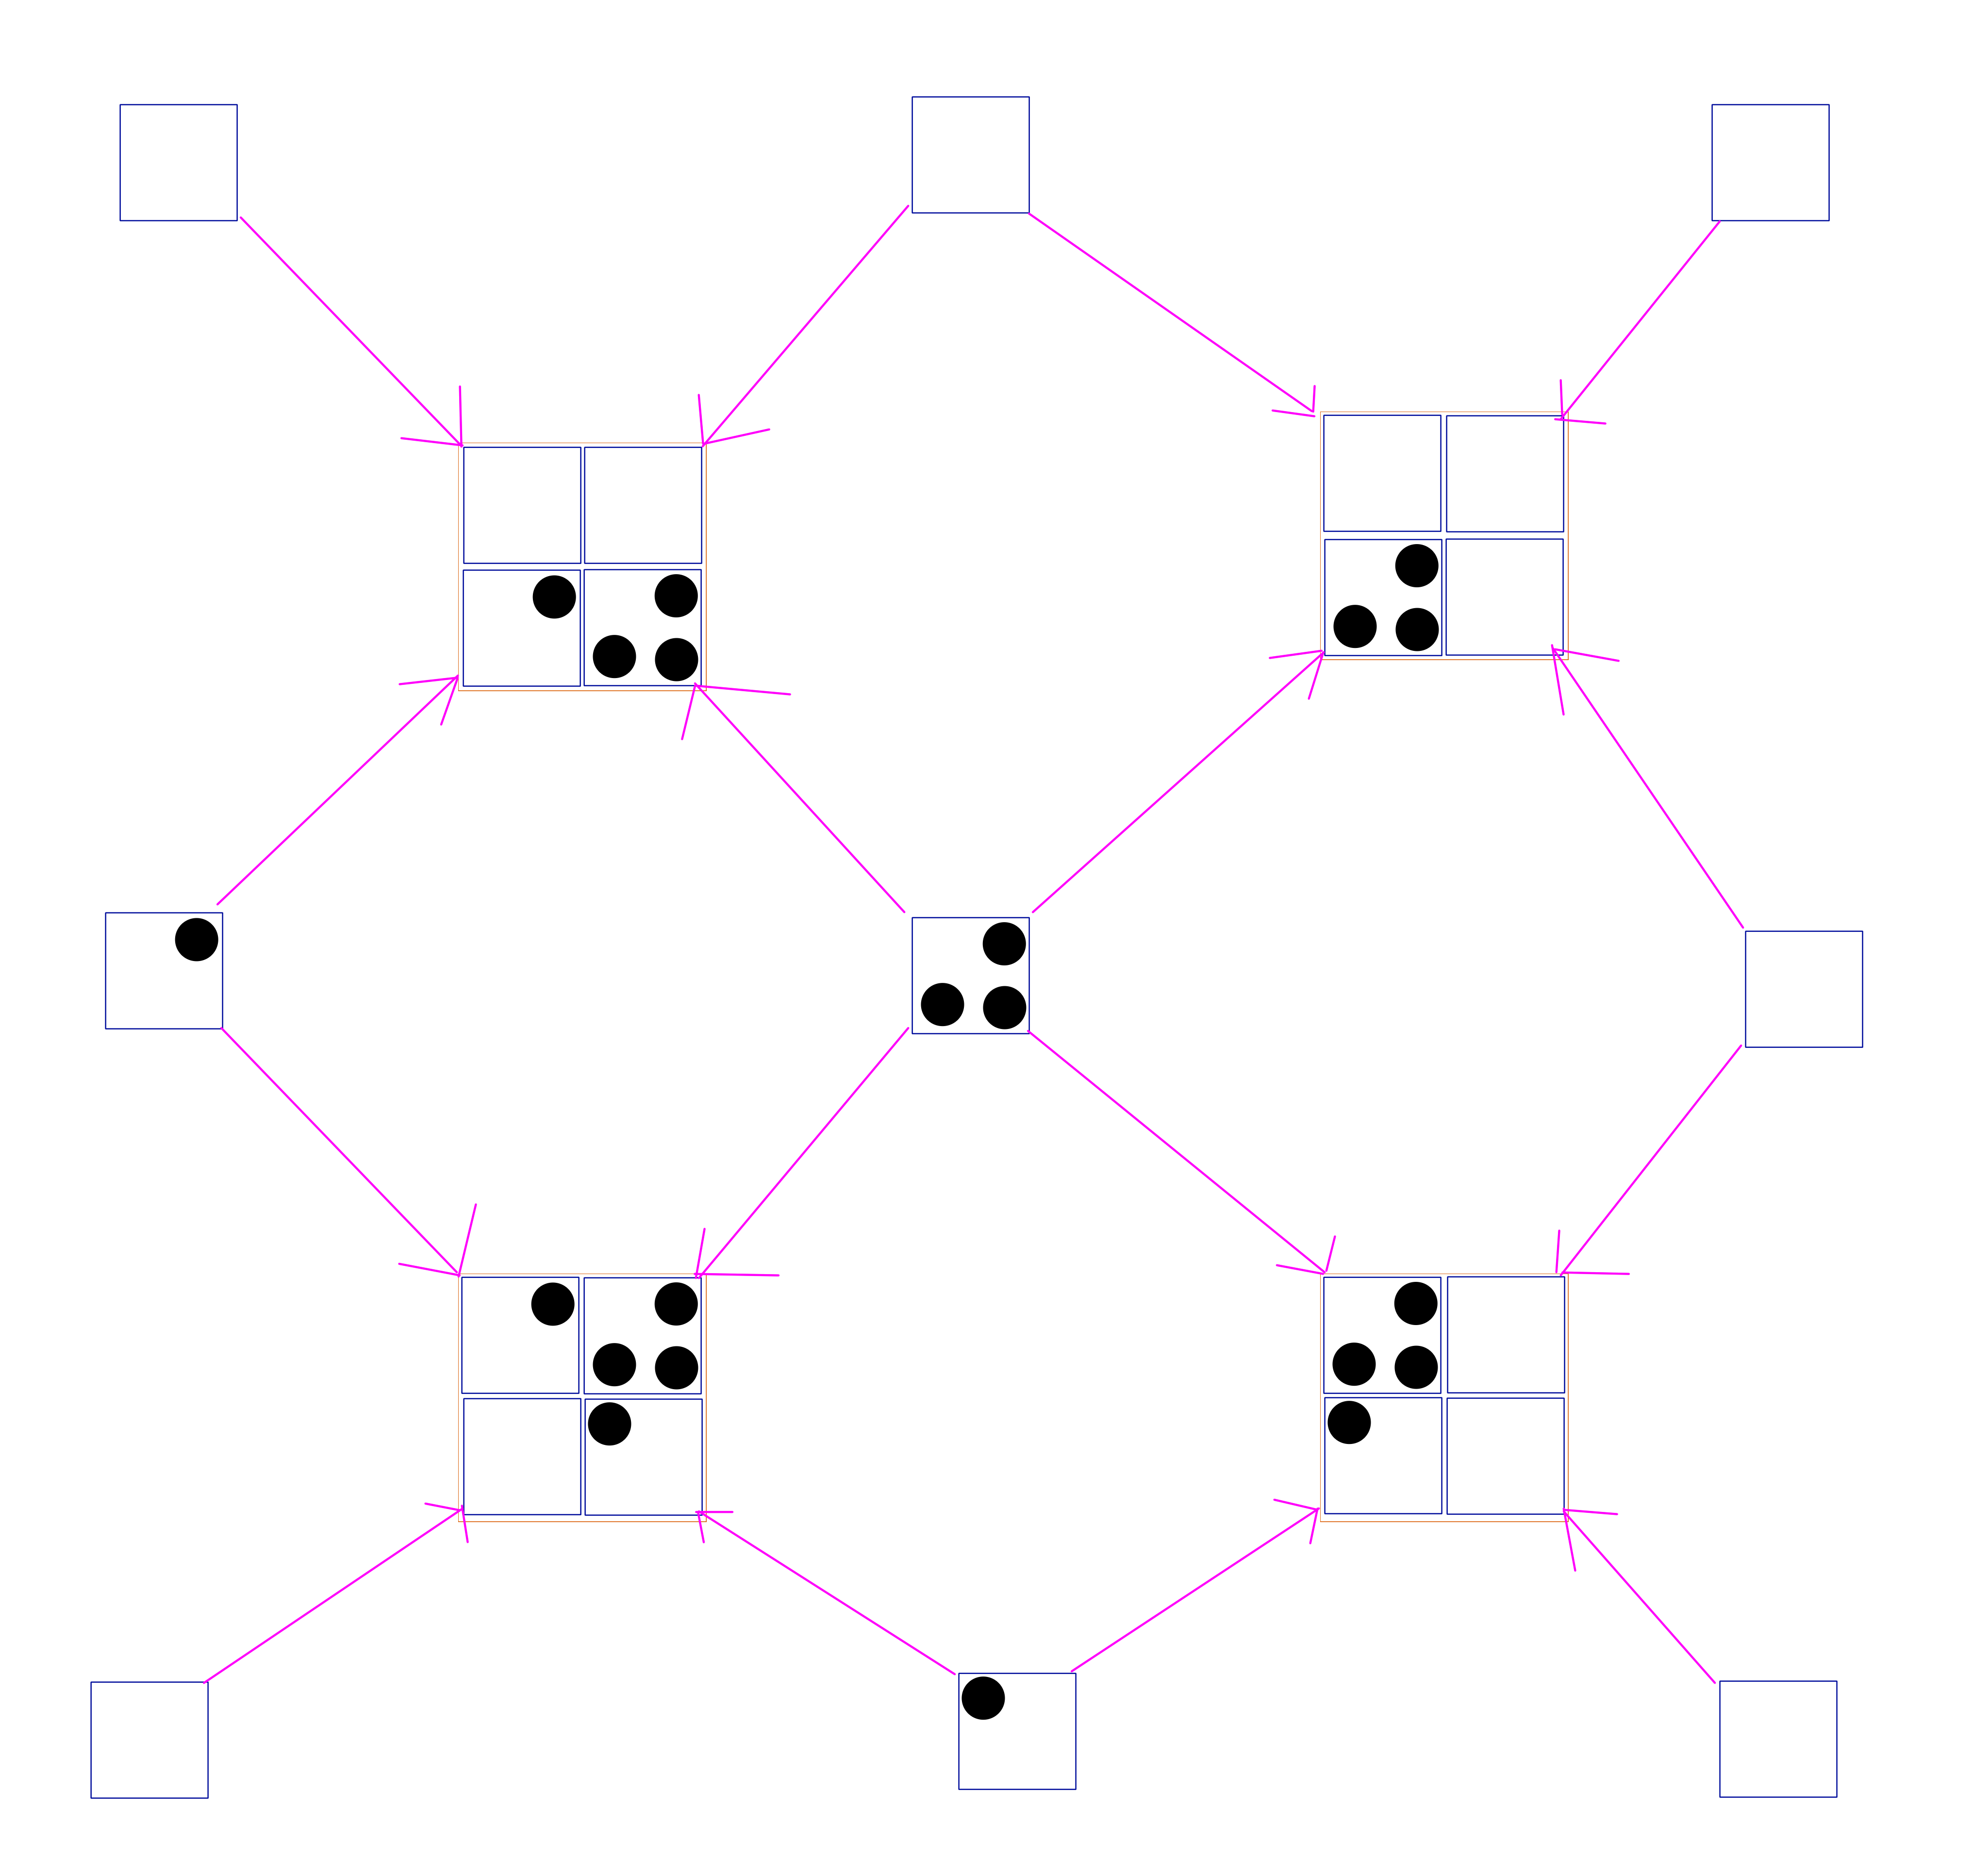
\includegraphics[scale=0.1]{images/imgHashlife/HashlifeStep3.png}
        \caption{Troisième étape de l'algorithme de Hashlife, ensuite on applique le même algorithme que almost hashlife sur les 4 nodes générées.}
\end{figure}
Pourtant un tel algorithme ne semble pas être bénéfique pour la performance car on calcule beaucoup de nodes déjà calculées, Cependant l'utilisation de la memoization va nous permettre d'exploiter ces propriétés sans trop affecter la durée entre deux changements de génération. Ainsi la première génération de Hashlife peux prendre beaucoup de temps a calculer (dans notre projet cela peux prendre entre 10 secondes et 5min dans le modele \textbf{metacellgalaxy.rle}), mais dès qu'assez de nodes ont été memoizées la performance devient difficile a représenter, alors que l'on calculait des dizaines de milliers de génération en une seconde avec almost-Hashlife on peut maintenant calculer si vite que le nombre de génération est difficile a retenir dans un entier long non-signé dont la limite est \textbf{18,446,744,073,709,551,615} , sans compter le fait qu'on peux augmenter la taille de l'arbre car plus l'arbre est gros plus on saute de générations! Il a donc été nécessaire d'imposer un court délai (\textit{5ms}) entre deux saut de génération de Hashlife afin que l'on puisse observer ce que fait l'algorithme. 

Ainsi Hashlife nous permet de simuler le jeu de la vie de la manière la plus rapide possible, que pouvons nous faire avec?

\subsection{résultats}
Voici une section un peux plus intéressante! Tout les modèles que nous allons vous montrer sont importés et simulés dans notre projet grâce a un lecteur RLE vous en trouverez plus d'informations dans la partie interface graphique. Tous ces modèles proviennent de \href{https://conwaylife.com/wiki/}{ce site}. Cessons donc parler d'algorithmes voyons voir se qu'ils ont dans le ventre:
\begin{figure}[H]
        \center
        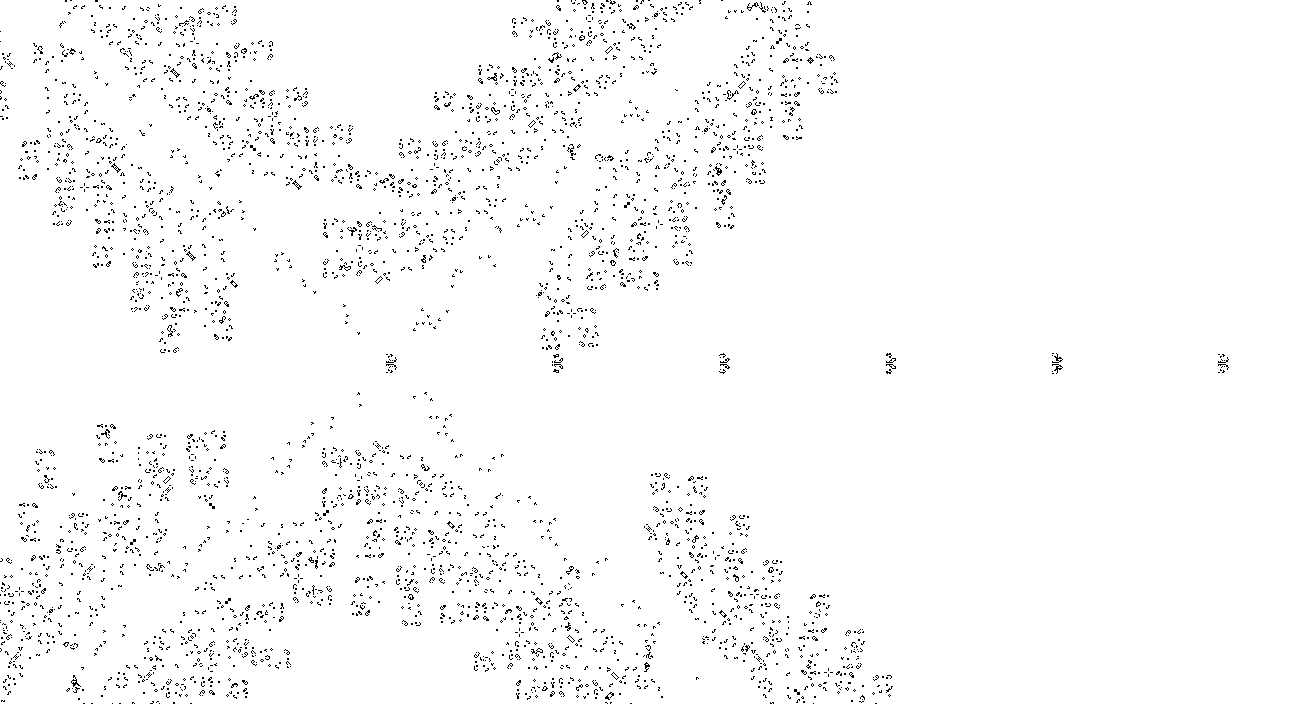
\includegraphics[scale=0.3]{images/imgHashlife/biggun.png}
        \caption{un pistolet a gros vaisseaux, almost hashlife suffit pour voir ce modele en action}
\end{figure}


\begin{figure}[H]
        \center
        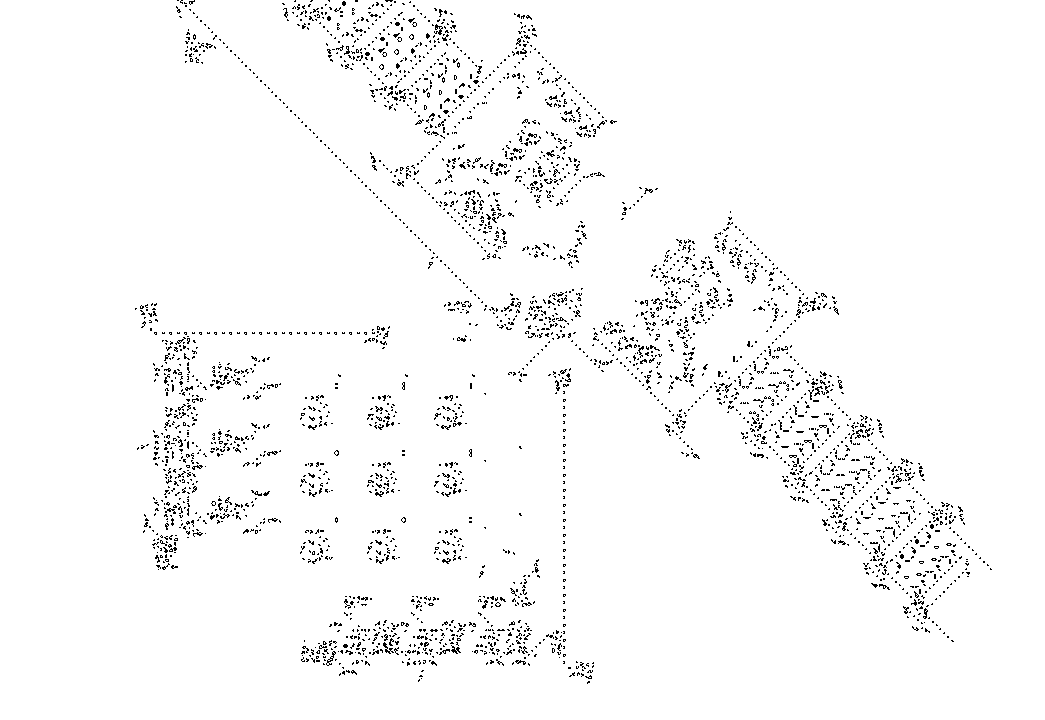
\includegraphics[scale=0.3]{images/imgHashlife/turingmachine.png}
        \caption{une machine de turing qui calcule les nombres premiers,
        on peux voir la sortie de celle ci en bas a gauche en flux de gliders}
\end{figure}

Les modèles suivants sont visionnables en temps réel grâce a hashlife

\begin{figure}[H]
        \center
        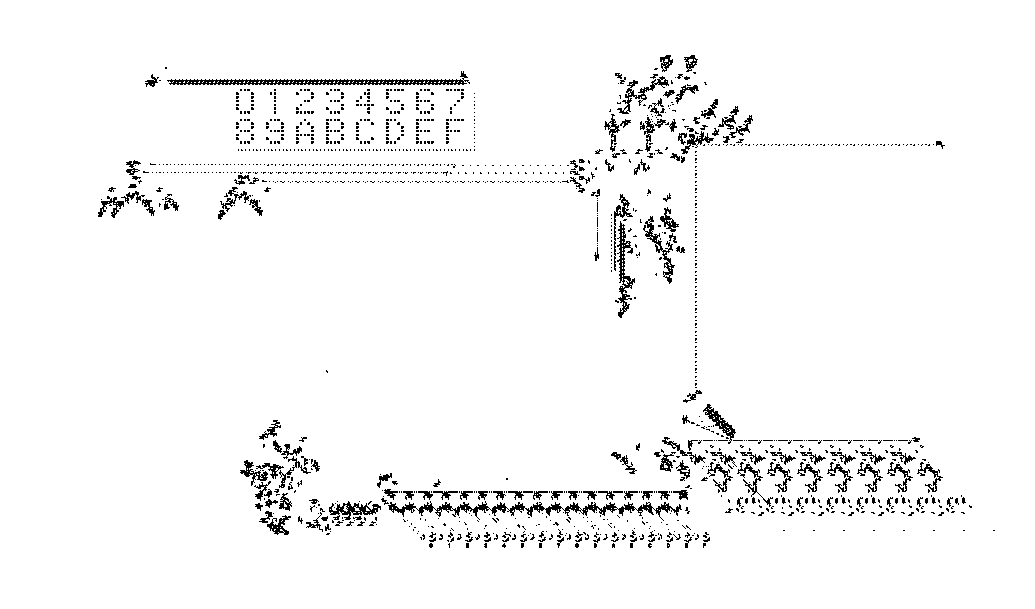
\includegraphics[scale=0.3]{images/imgHashlife/display.png}
        \caption{un affichage de lettres et chiffres on peux le voir afficher en temps réel chaque ligne de l'affichage. La première génération peux prendre \textit{45s}}
\end{figure}

\begin{figure}[H]
        \center
        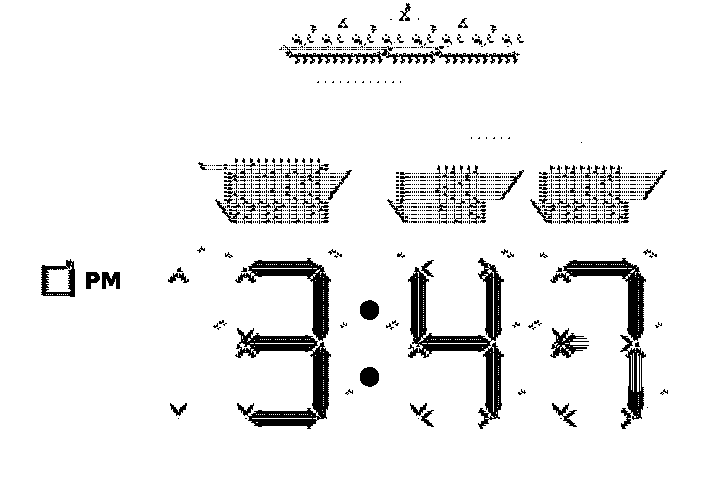
\includegraphics[scale=0.3]{images/imgHashlife/clock.png}
        \caption{une horloge digitale on peux la voir changer d'heure la première génération peux prendre \textit{1min20}}
\end{figure}

Et un dernier pour la route, et aussi le plus impressionnant!
\begin{figure}[H]
        \center
        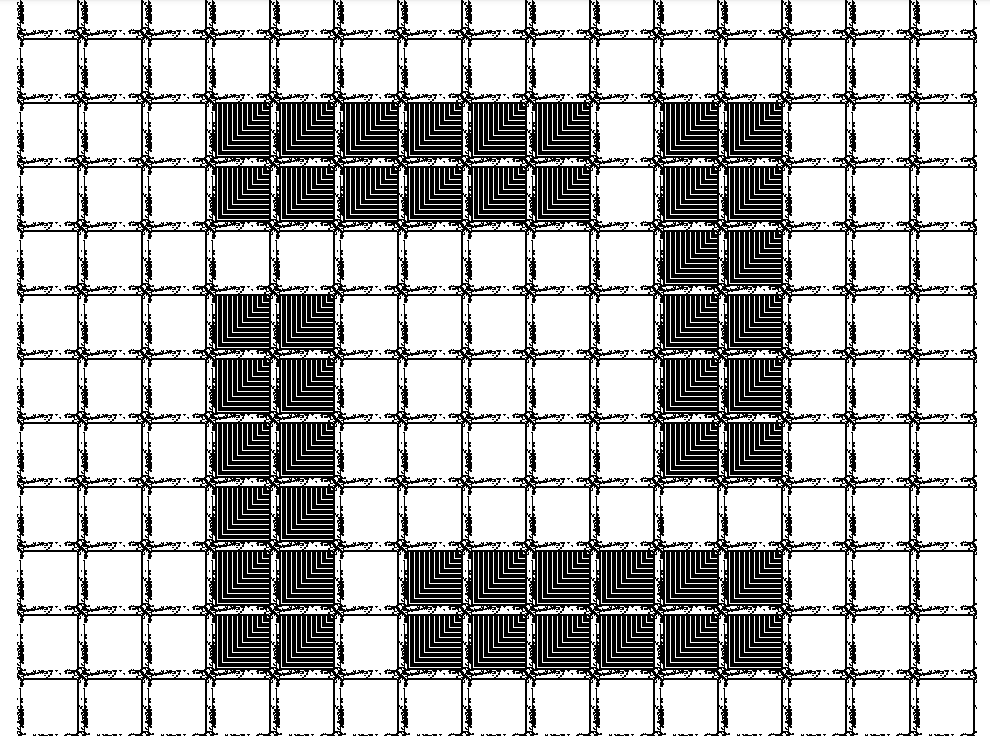
\includegraphics[scale=0.3]{images/imgHashlife/metacellgalaxy.png}
        \caption{le saint graal, le jeux de la vie dans le jeu de la vie grâce aux metacells, ici la galaxie de Kok la première génération peux prendre environ \textit{3-5min}, ce pattern est très dur a simuler sur mon petit laptop}
\end{figure}

Voila qui conclus cette explication de Hashlife.


\section{Interface Graphique}
\par L'interface graphique de notre application se décompose en 3 composants principaux :
\begin{itemize}
    \item Le Menu
    \item La fenêtre principale de l'application
    \item La fenêtre de chargement d'un modèle
\end{itemize}
\subsection{Menu}
\par Le Menu est la page d'accueil de l'application, il sert à choisir le type d'automate cellulaire souhaité pour la simulation de notre "Game of life". Le choix de l'automate cellulaire ce fait grâce aux boutons :
\begin{itemize}
    \item \textbf{Hashlife} bouton (initialise un automate cellulaire utilisant l'algorithme hahslife)
    \item \textbf{Margolus} bouton (initialise un automate cellulaire utilisant les algorithmes de margolus)
    \item \textbf{Neural} bouton (initialise un automate cellulaire utilisant les algorithmes neuronaux)
\end{itemize}

\begin{figure}[H]
    \centering
    
\includegraphics[width=0.5\textwidth]{images/imgInterface/boutons.png}
    \caption{Bouton Hashlife du menu}
    \label{fig:hashlife bouton}
\end{figure}

\par Chaque bouton est accompagné sur sa droite d'un bouton d'information. Chaque bouton ouvre une fenêtre pop-up contenant un lien qui renvoie vers un site permettant d'avoir plus d'informations sur l'option à sa gauche.

\begin{figure}[H]
    \centering
    
\includegraphics[width=0.5\textwidth]{images/imgInterface/boutonInformation.png}
    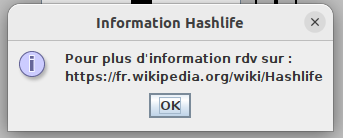
\includegraphics[width=0.5\textwidth]{images/imgInterface/popup.png}
    \caption{Bouton d'information de Hashlife}
    \label{fig:bouton info}
\end{figure}

\subsection{Fenêtre principale}
\par La fenêtre principale permet l'affichage de l'automate cellulaire ainsi que son contrôle grâce de multiples boutons présent sur une \textbf{JToolBar} : la barre d'options

\subsubsection{Barre d'option}

\par La barre d'option contient 10 boutons :
\begin{itemize}
    \item \textbf{Home} (permet de revenir dans le menu pour changer d'automate cellulaire)
    
    \item \textbf{Move} (permet de ce déplacer dans l'affichage de l'automate et de zoomer)
    
    \item \textbf{Secret} (je vous laisse découvrir le secret par vous même)
    
    \item \textbf{Rule} (affiche la règle courante suivit par l'automate cellulaire)
    
    \item \textbf{Choix rules} (un menu déroulant contenant les différentes règles que l'automate peut suivre (change en fonction de l'automate))
    
    \item \textbf{Play} (permet de lancer/mettre en pause la simulation de l'automate cellulaire)
    
    \item \textbf{Random} (permet de remplir l'automate cellulaire aléatoirement)
    
    \item \textbf{Clear} (permet de vider l'automate cellulaire)
    
    \item \textbf{Speed} (permet d'accélérer la vitesse de la simulation, il n'est disponible que si l'automate utilise l'algorithme hashlife)
    
    \item \textbf{Modele} (un menu déroulant contenant différents modèle importable du jeu de la vie (les modèles changent en fonction de l'automate initialisé)
\end{itemize}

\begin{figure}[H]
    \centering
    
\includegraphics[width=1\textwidth]{images/imgInterface/optionBar.png}
    \caption{Barre d'options}
    \label{fig:barre d'options} 
\end{figure}

\subsubsection{Affichage automate}
\par Comme dis précédemment l'affichage automate affiche la simulation du jeu de la vie en cours. Dans cette affichage vous pouvez cliquer affin d'ajouter une cellule vivante (représenter par un pixel noir) sur l'endroit cliqué. Pour se déplacer et zoomer dans l'affichage c'est très simple :

\begin{itemize}
    \subsubsection{Déplacement}
    \item \textbf{z/Z} déplacement vers l'avant
    \item \textbf{q/Q} déplacement vers la gauche
    \item \textbf{d/D} déplacement vers la droite
    \item \textbf{s/S} déplacement vers l'arrière
    \subsubsection{Zoom}
    \item \textbf{a/A} zoom +
    \item \textbf{e/E} zoom -
\end{itemize}{}

\begin{figure}[H]
    \centering
    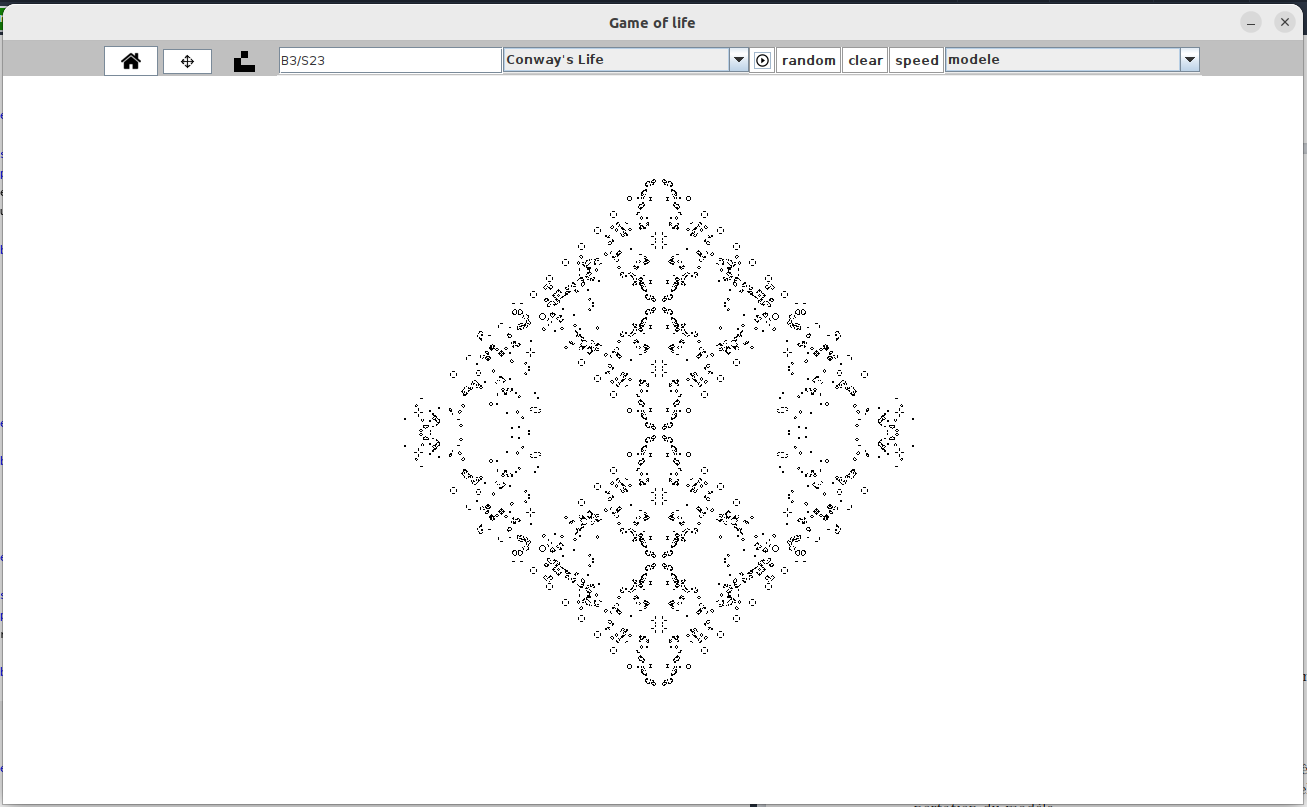
\includegraphics[width=0.5\textwidth]{images/imgInterface/simulation2.png}
    \caption{Affichage d'une simulation}
    \label{fig:simulation} 
\end{figure}

\subsection{Fenêtre de chargement}
\par Lorsque l'on importe un nouveau modèle alors la fenêtre de chargement s'ouvre et une barre de progression est affiché. La barre selon le niveau d'importation du modèle.

\begin{figure}[H]
    \centering
    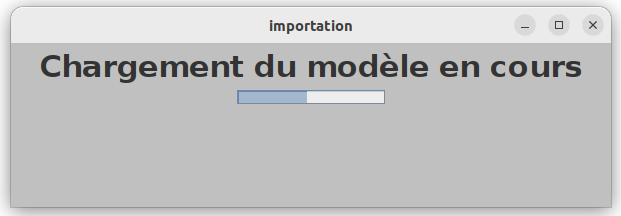
\includegraphics[width=0.5\textwidth]{images/imgInterface/chargement.png}
    \caption{Fenêtre de chargement}
    \label{fig:chargement} 
\end{figure}

\section{Architecture du Projet}
Pour notre Projet, nous avons créé plusieurs package différents afin d'avoir un espace de travail ordonné et rigoureux.
Ainsi nous avons un package \textbf{build} contenant toute les classes après compilation, un package \textbf{doc} contenant toute la javadoc compilé, un package \textbf{lib} contenant la librairie afin d'exécuter correctement les tests, un package \textbf{ressource} qui contient les package CSV, img et RLE contenant respectivement les fichiers au format .csv, .png et .rle et enfin nous avons le package \textbf{src} qui contient tout notre code. 
\begin{figure}[htp]
\centering
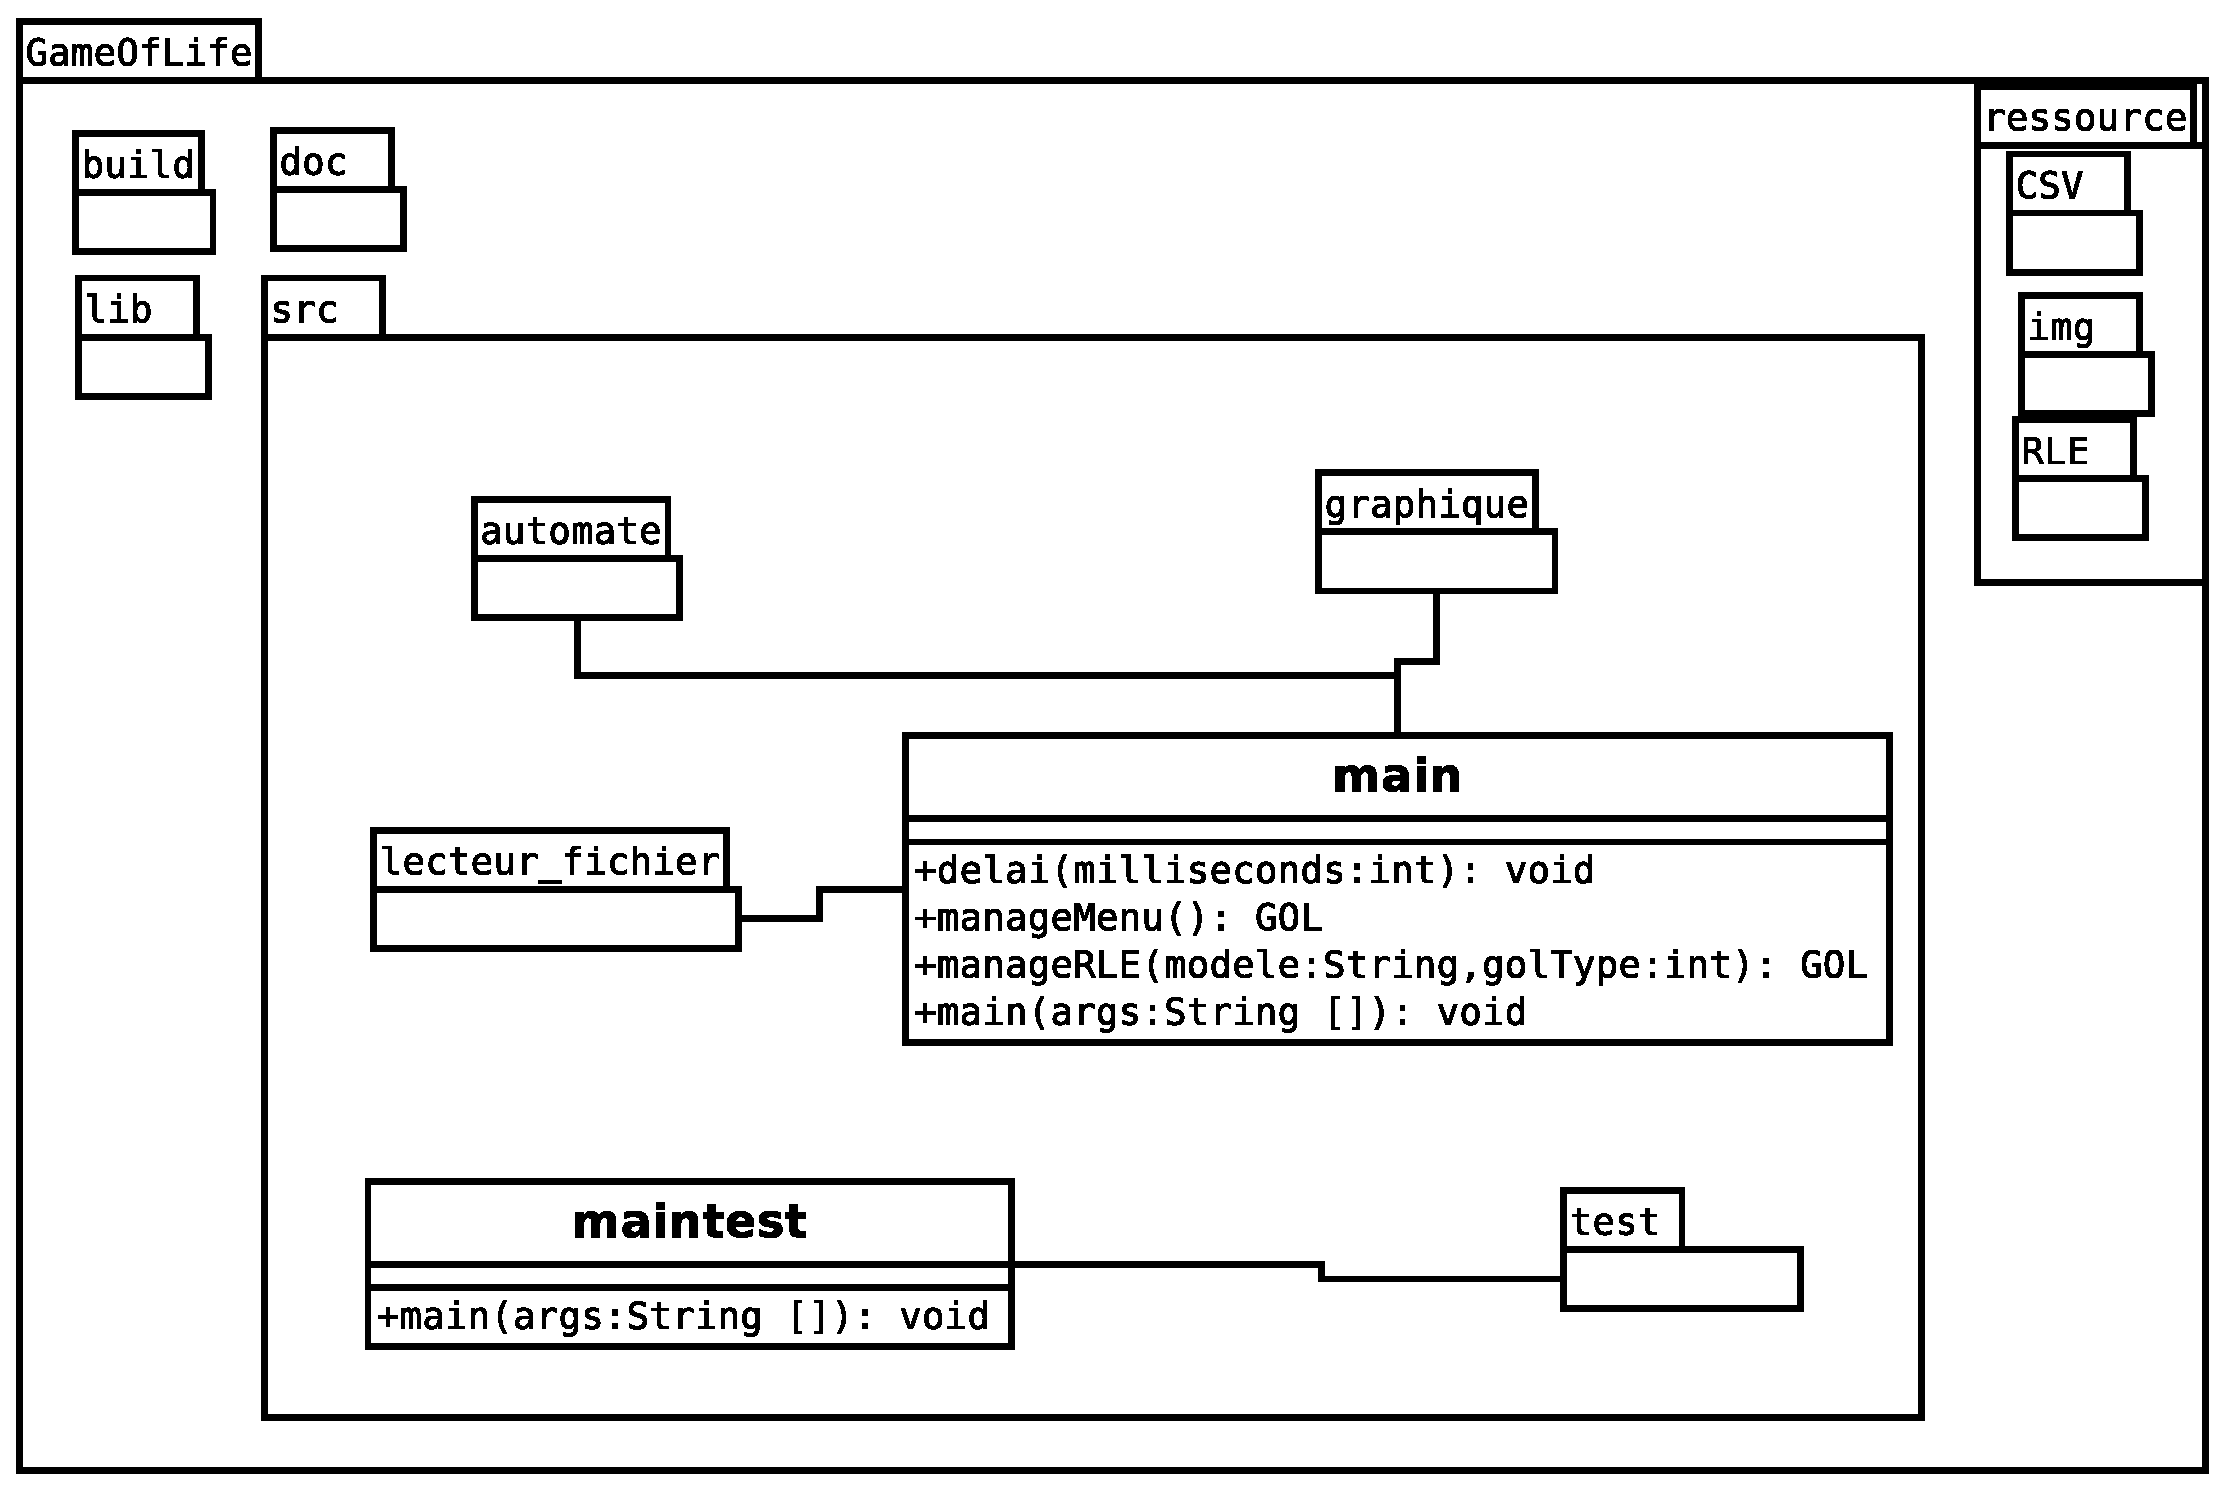
\includegraphics[scale=0.35]{images/Diagramme/Projet.eps}
\caption{\label{fig:GameOfLife}Illustration du package GameOfLife}
\end{figure}

\par Dans le package src nous avons différents package ainsi que les deux classes main : \begin{itemize}
    \item La classe \textbf{main} qui lance le jeu de la vie.
    \item La classe \textbf{maintest} qui lance tout les tests présents dans le package test et affiche la réussite ou l'échec de chacun.
\end{itemize}
\par Parmi les différents package nous avons les quatre suivants : \begin{itemize}
    \item Le package \textbf{automate}
    \item Le package \textbf{graphique}
    \item Le package \textbf{lecteur fichier}
    \item Le package \textbf{test}
\end{itemize}
\subsection{Package Automate}

\par Le package \textbf{automate} va initialiser les différentes versions du jeu de la vie ou de l'automate cellulaire. Il est composé de deux sous-package : \begin{itemize}
    \item Le package \textbf{gridlife} initialisant les différentes versions d'automates cellulaires sur une grille.
    \item Le package \textbf{hashlife} initialisant le jeu de la vie sur un ensemble de quadtree.
\end{itemize}

\par Ce package compte aussi deux classes abstraites et une interface qui initialise les méthodes communes au deux package.
La classe abstraite \textbf{GOL} généralise les variables communes et les fonction utilisées dans les classes qui l'héritent (\textbf{GOLqTree}, \textbf{GOLGrille}), cette classe va être utilisée dans l'interface et le main afin de pouvoir changer rapidement d'instance de \textbf{GOL} et initialiser les modèles RLE. \\
La classe abstraite \textbf{Decode} va servir a décoder les règles du jeu de la vie ou de l'automate cellulaire. Elle contient les règles ainsi qu'une méthode abstraite qui doit vérifier si les règles sont valides ainsi qu'un accesseur. Cette classe sera hérité par une classe pour chaque instance différente de \textbf{GOL} : 
\begin{itemize}
    \item la classe \textbf{DecodeqTree} dans le package hashlife qui va décoder les règles de format standard du jeu de la vie (B.../S...) exemple : Conway's Life (premier jeu de la vie) a pour règles B3/S23 .
    \item la classe \textbf{DecodeGrilleLifeLike} dans le package gridlife qui va décoder les règles de format (././././././././././././././././) prenant 15 chiffres entier entre 0 et 15 (inclus) qui est utilisé pour les algorithmes neuraux.
    \item la classe \textbf{DecodeGrilleMargolus} dans le package gridlife qui va décoder les règles de format (././././././././) prenant 8 chiffres entre 0 et 1 qui est utilisé pour les voisinages de Margolus.
\end{itemize}
\begin{figure}[htp]
\centering
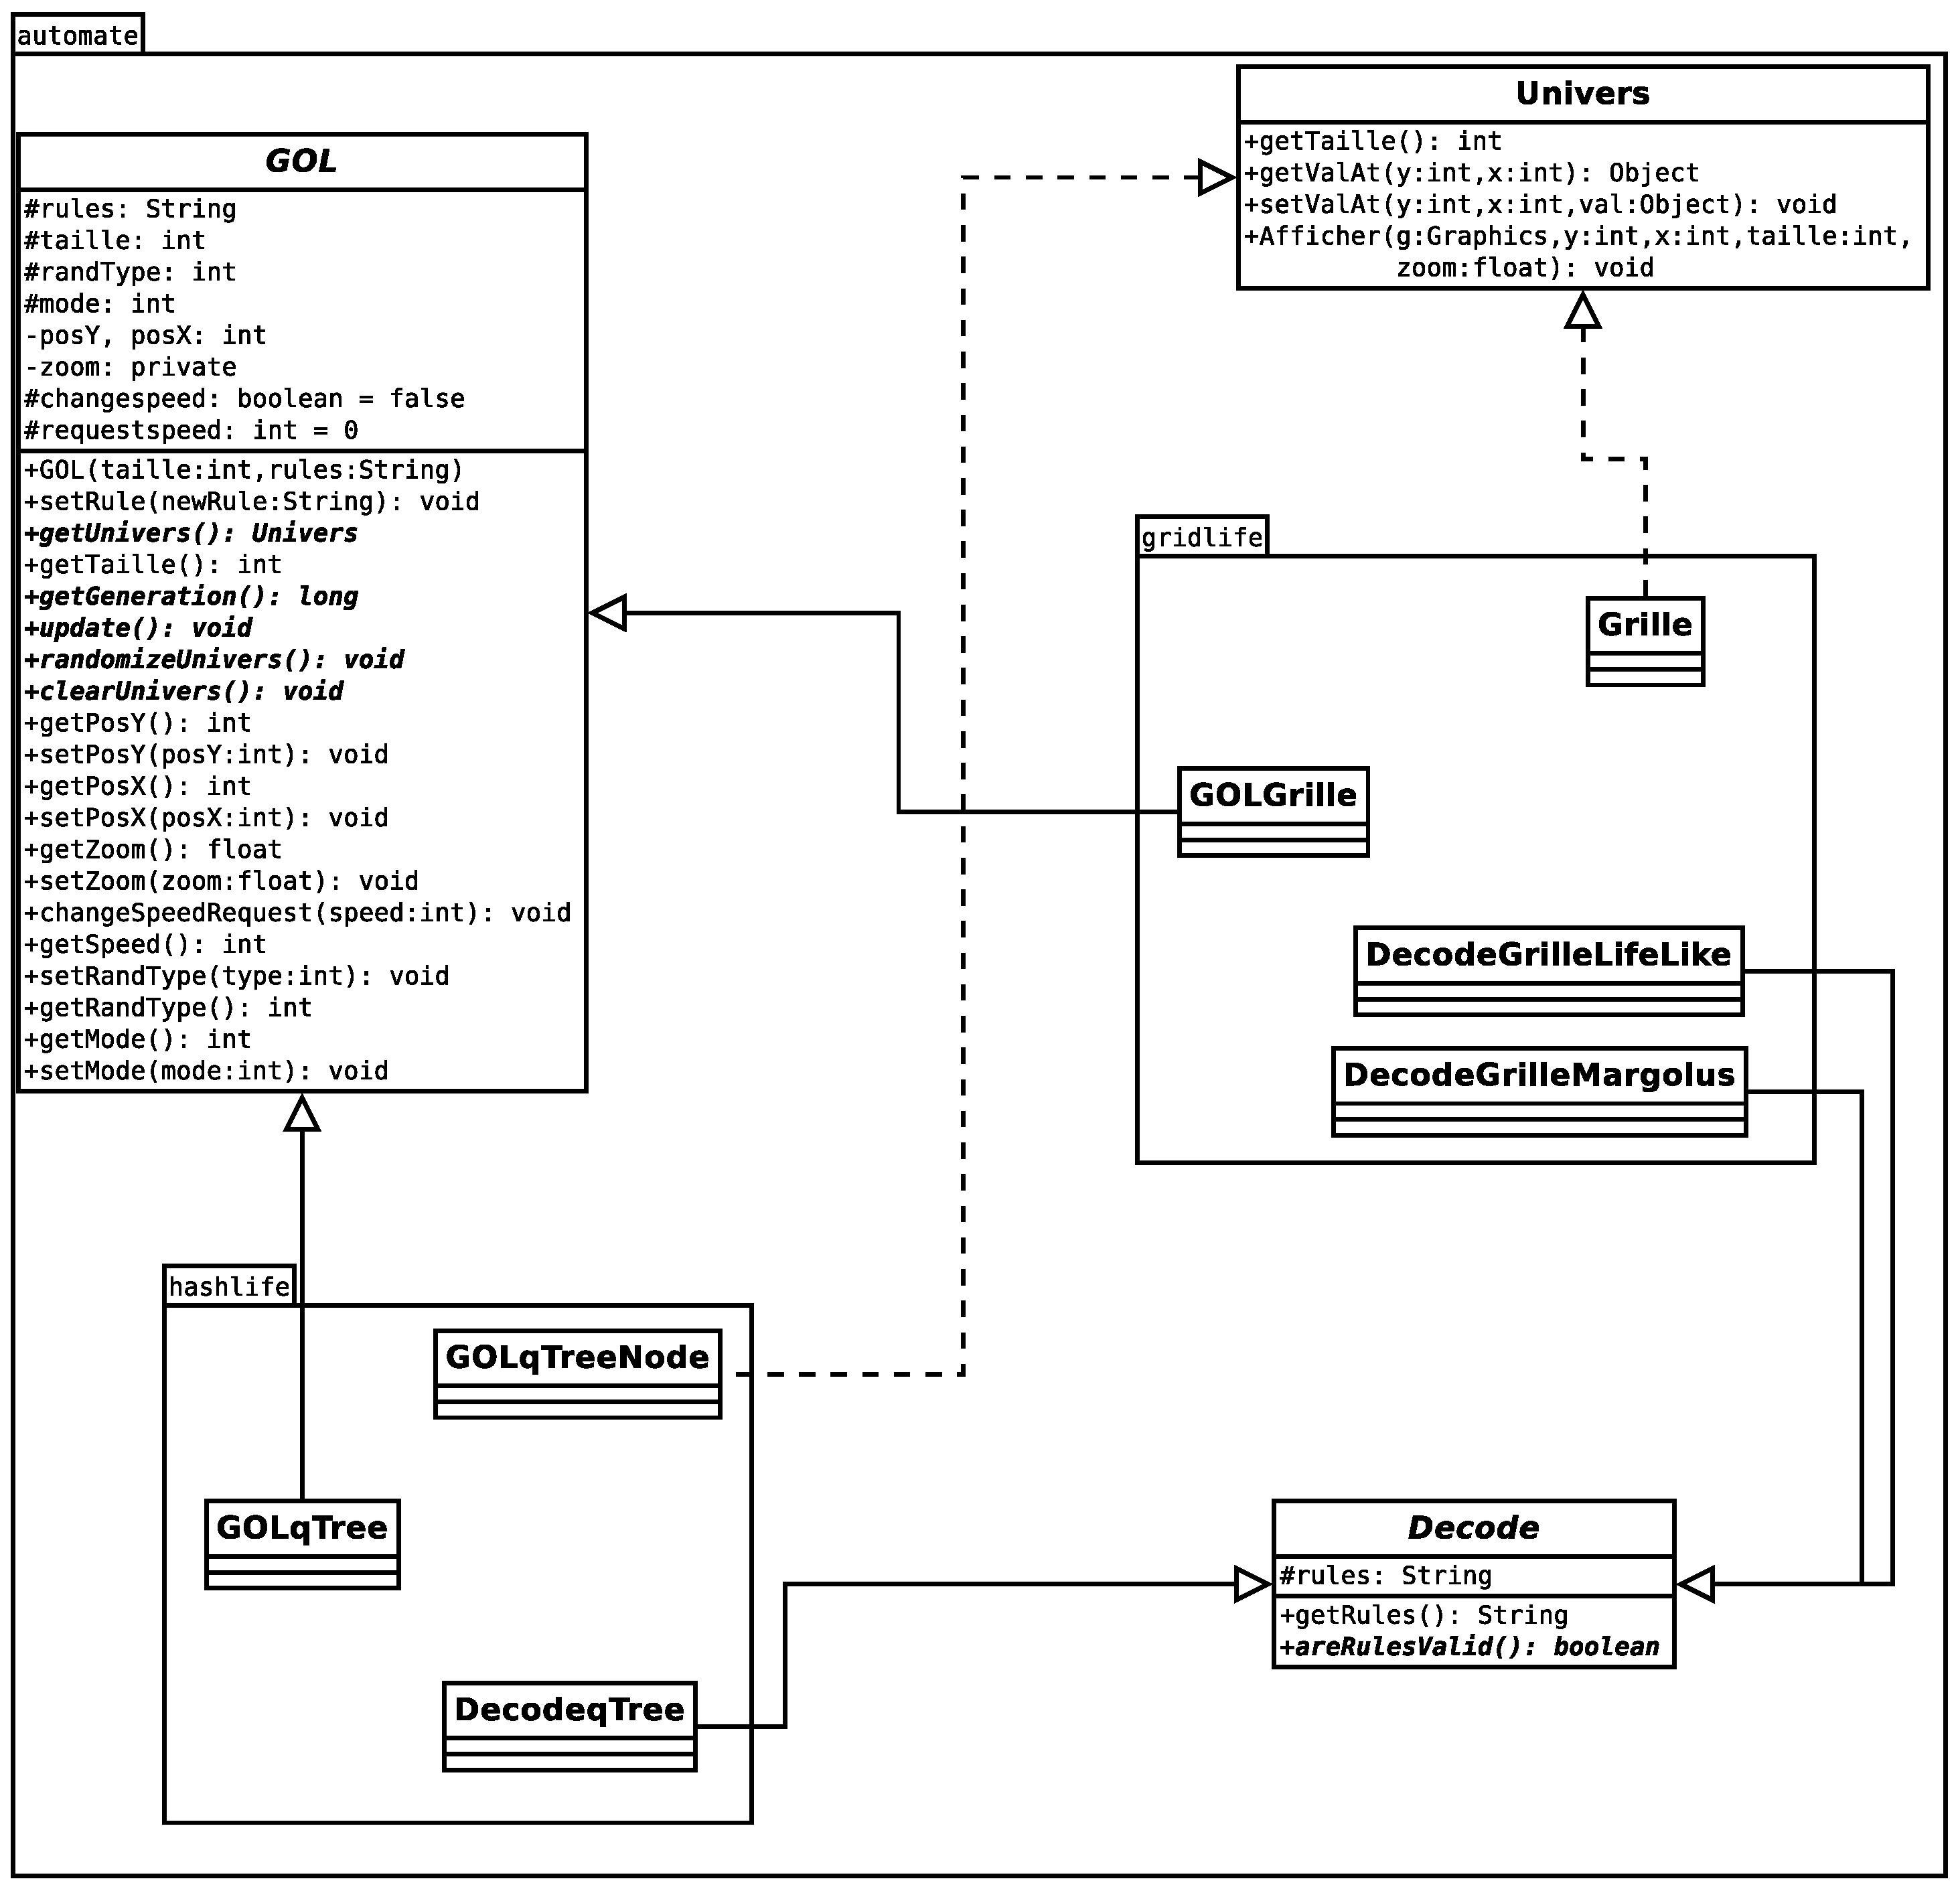
\includegraphics[scale=0.25]{images/Diagramme/package_automate.eps}
\caption{\label{fig:Automate}Illustration du package automate}
\end{figure}
\par L'interface Univers va être implémentée par les "supports" du jeu de la vie ou des automates cellulaires. La classe \textbf{Grille} dans le package gridlife et la classe \textbf{GOLqTreeNode} dans le package hashlife. Cette interface va initialisé les accesseurs et modificateurs de valeur à une certaine coordonnée ainsi qu'une méthode permettant l'affichage sur un Graphics.
\subsubsection{package gridlife}
\par Le package gridlife va représenter les automates cellulaires sur grille. Il est composé des différentes classes héritant du package automate : \begin{itemize}
    \item la classe \textbf{Grille}
    \item la classe \textbf{GOLGrille}
    \item la classe \textbf{DecodeGrilleLifeLike}
    \item la classe \textbf{DecodeGrilleMargolus}
\end{itemize}

\begin{figure}[htp]
\centering
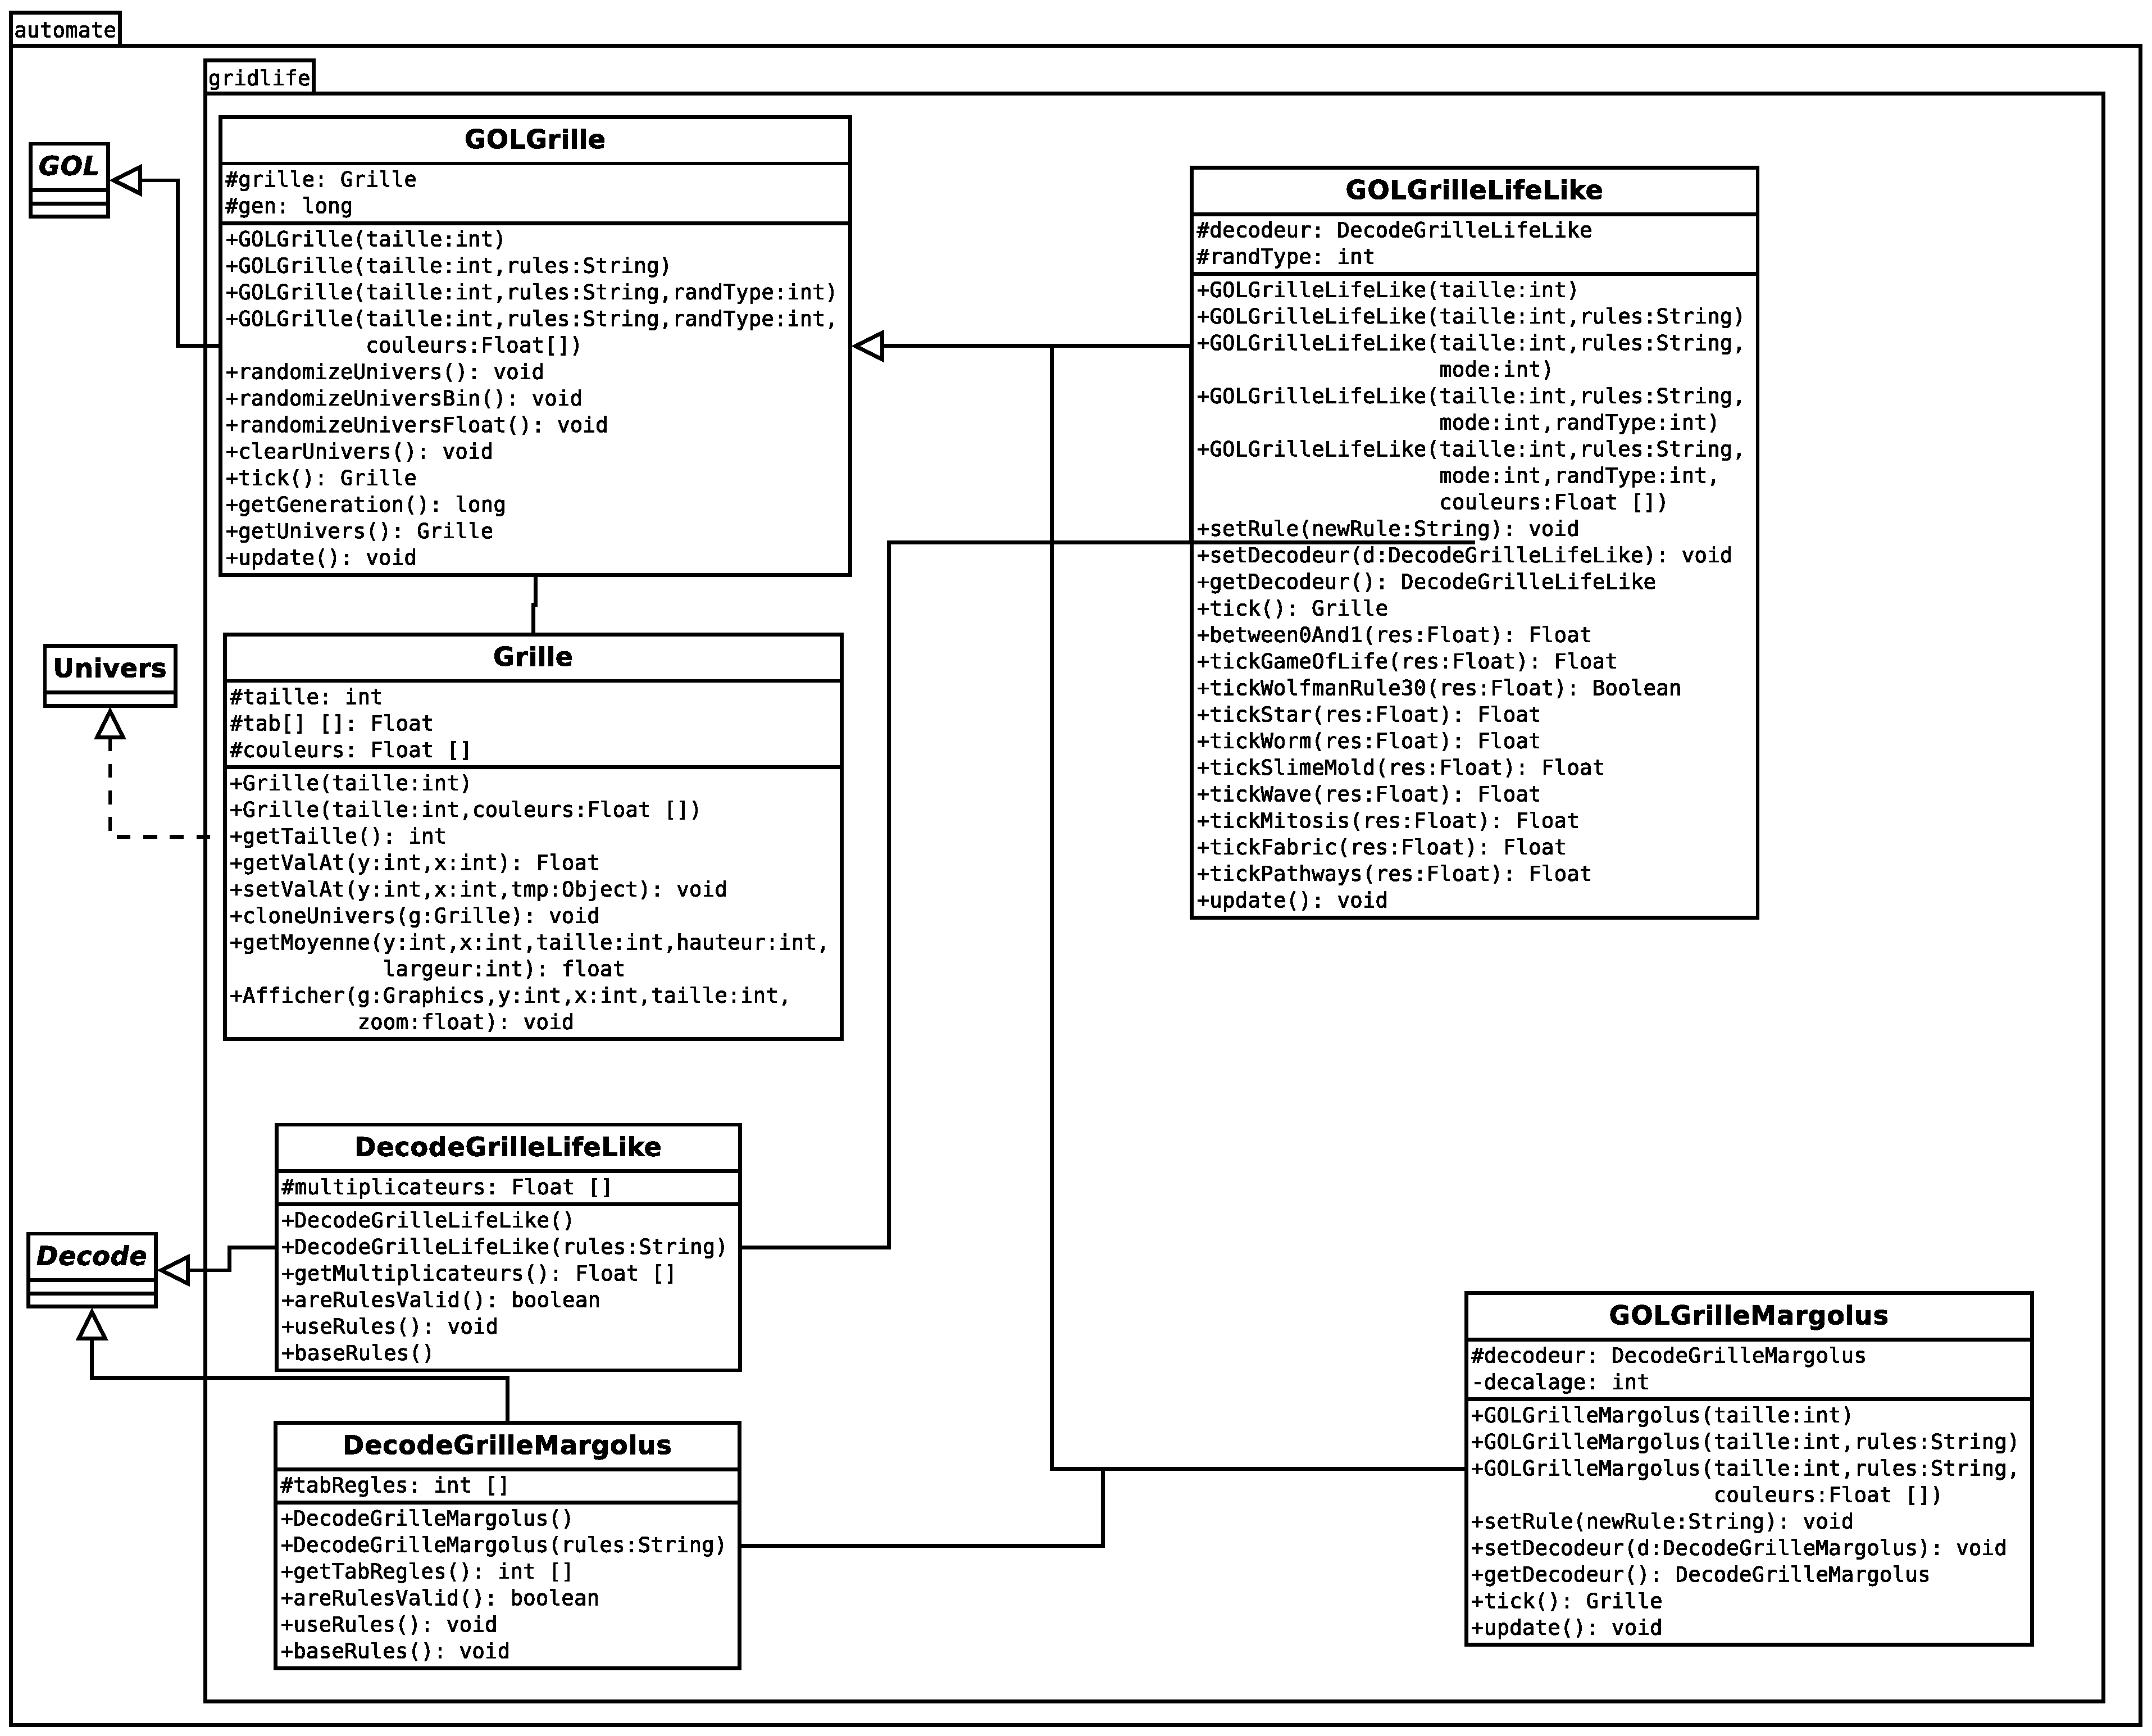
\includegraphics[scale=0.25]{images/Diagramme/package_automate_gridlife.eps}
\caption{\label{fig:Automate/gridlife}Illustration du package automate/gridlife}
\end{figure}
\par Il contient aussi les classes \textbf{GOLGrilleLifeLike} et \textbf{GOLGrilleMargolus} héritant de \textbf{GOLGrille} qui définissent et lancent les différentes versions des automates cellulaires et utilisent les différents décodeur respectivement les algorithmes neuraux et les voisinages de Margolus.
\subsubsection{package hashlife}
Le package hashlife regroupent toutes les classes permettant d'initialiser le jeu de la vie avec des quadtrees. Il est composé des différentes classes héritant du package automate :\begin{itemize}
    \item La classe \textbf{GOLqTreeNode}
    \item La classe \textbf{GOLqTree}
    \item La classe \textbf{DecodeQtree}
\end{itemize}
\begin{figure}[htp]
\centering
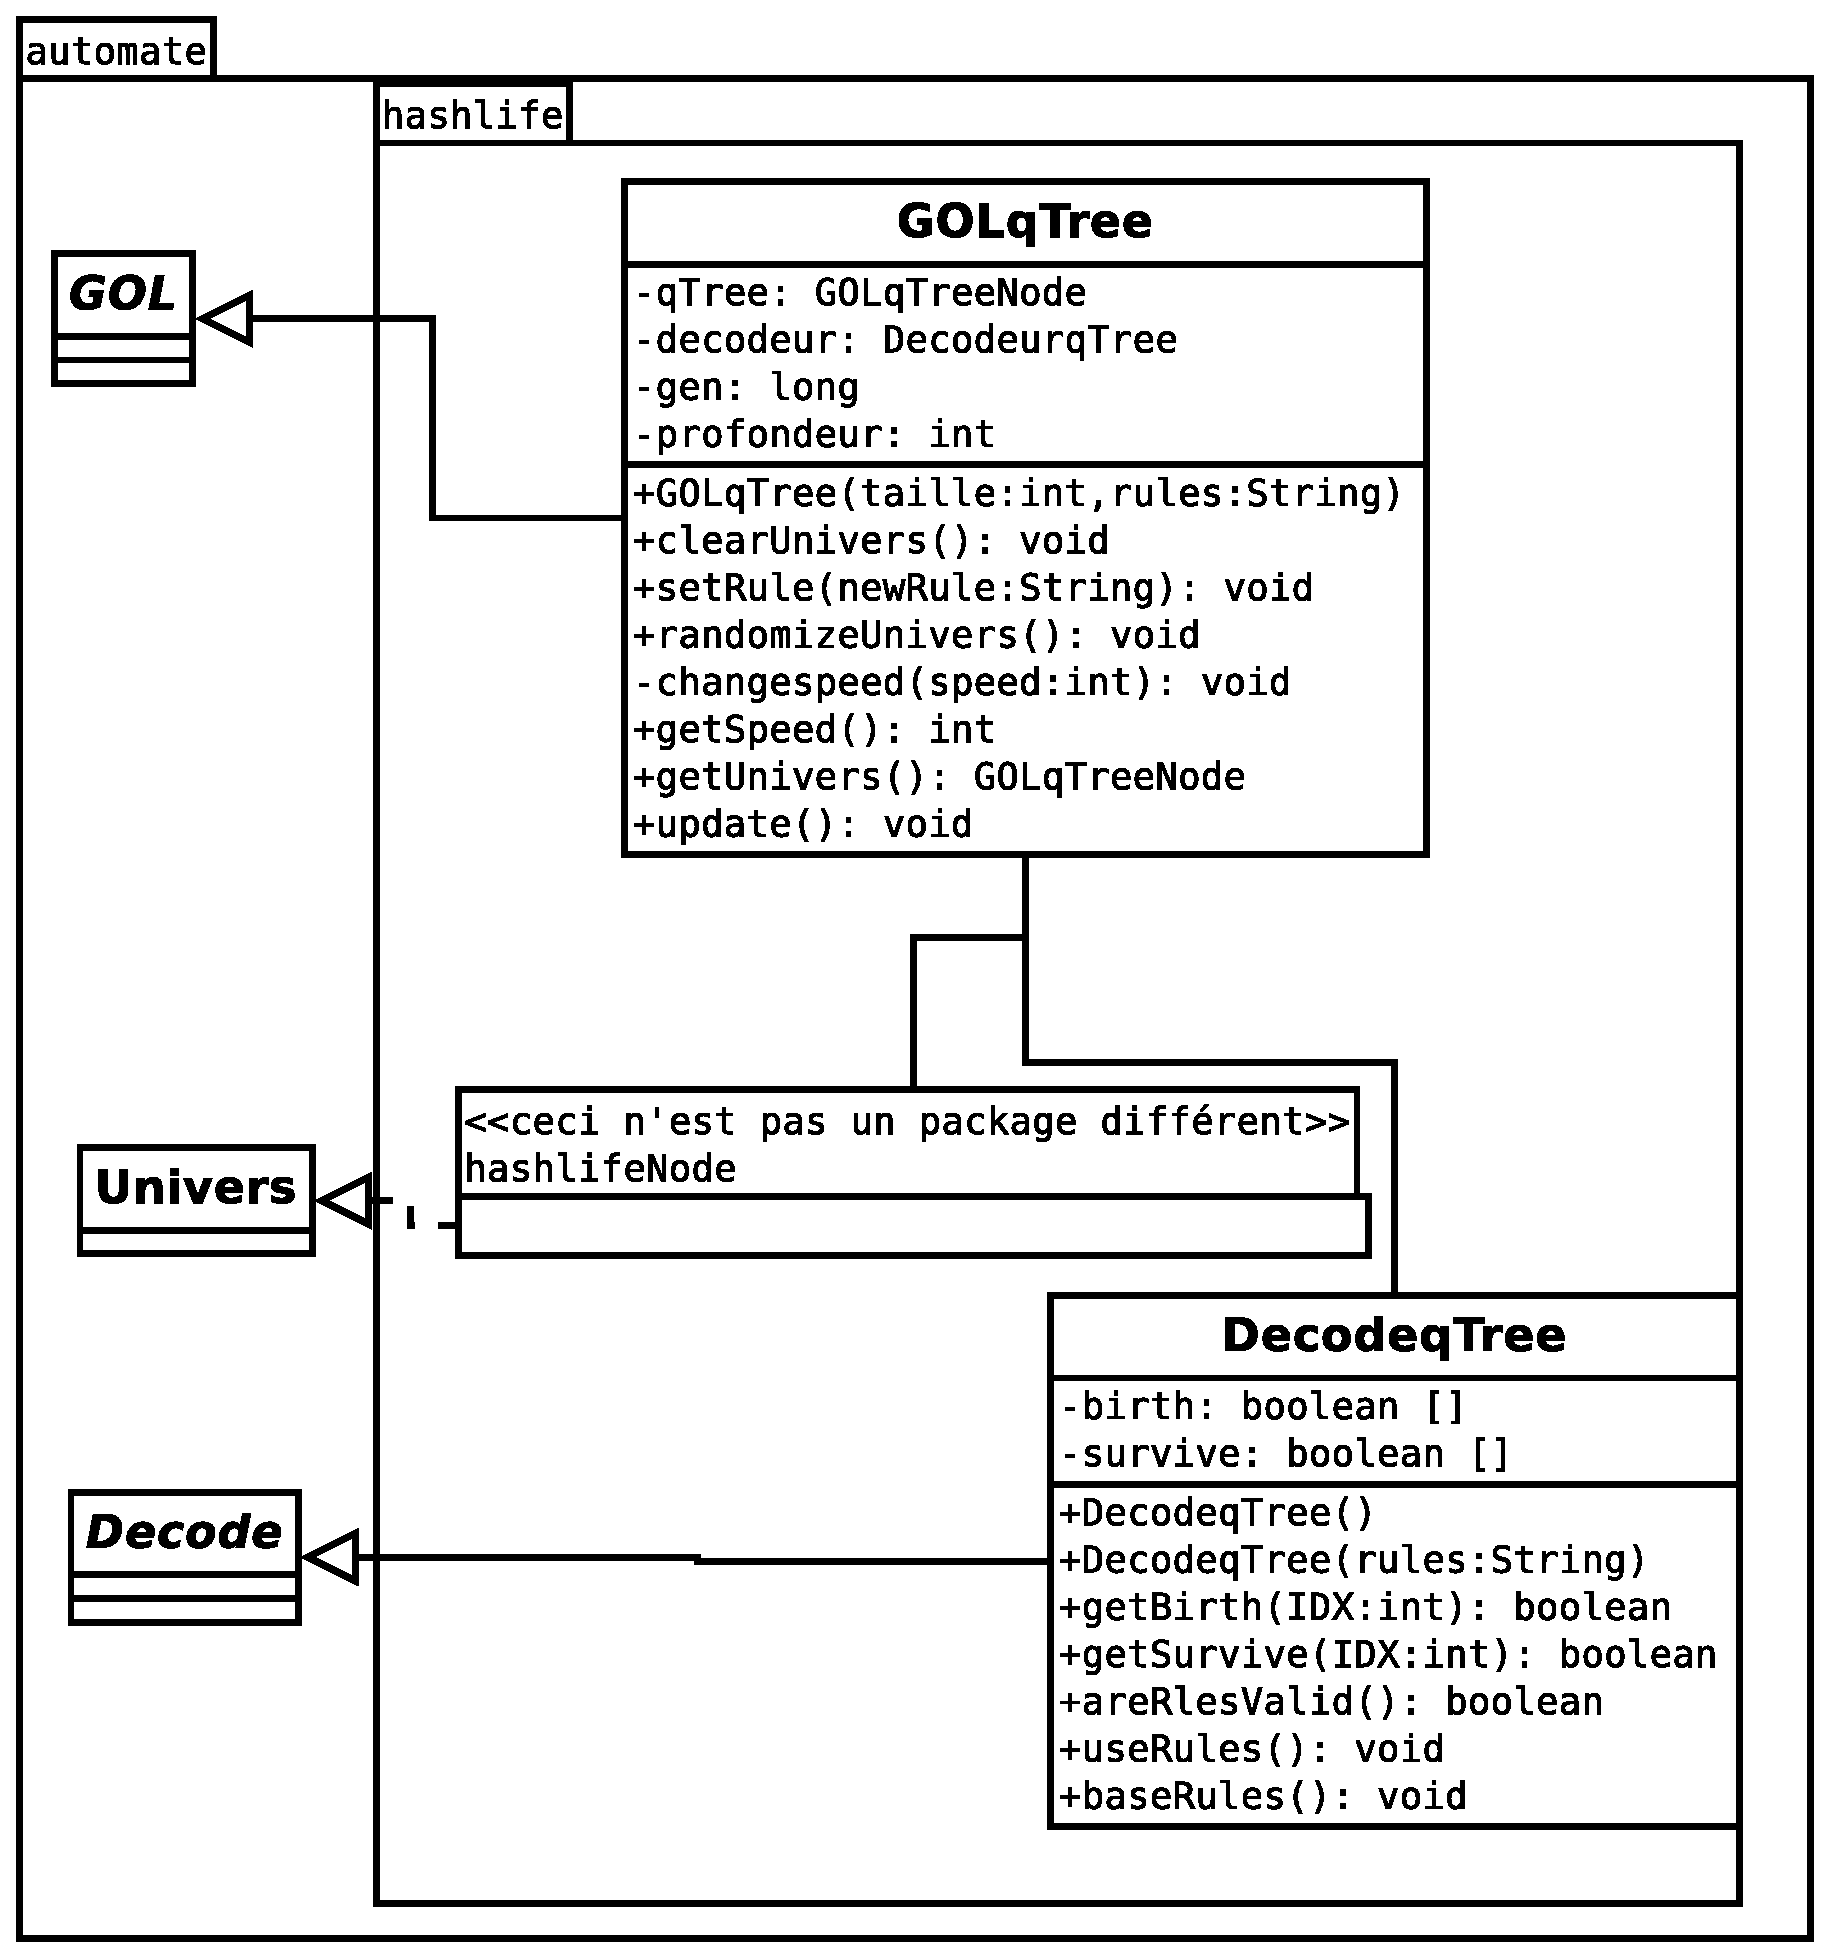
\includegraphics[scale=0.35]{images/Diagramme/package_automate_hashlife.eps}
\caption{\label{fig:Automate/hashlife}illustration du package automate/hashlife}
\end{figure}
\par Il contient également les classes permettant de placer le quadtree dans une hashMap (\textbf{CanonicalizedqTree}), une autre classe implémentant Almost-Hashlife (\textbf{MemoizedqTree}) ainsi qu'une classe implémentant hashlife (\textbf{HashlifeqTree}).
\begin{figure}[htp]
\centering
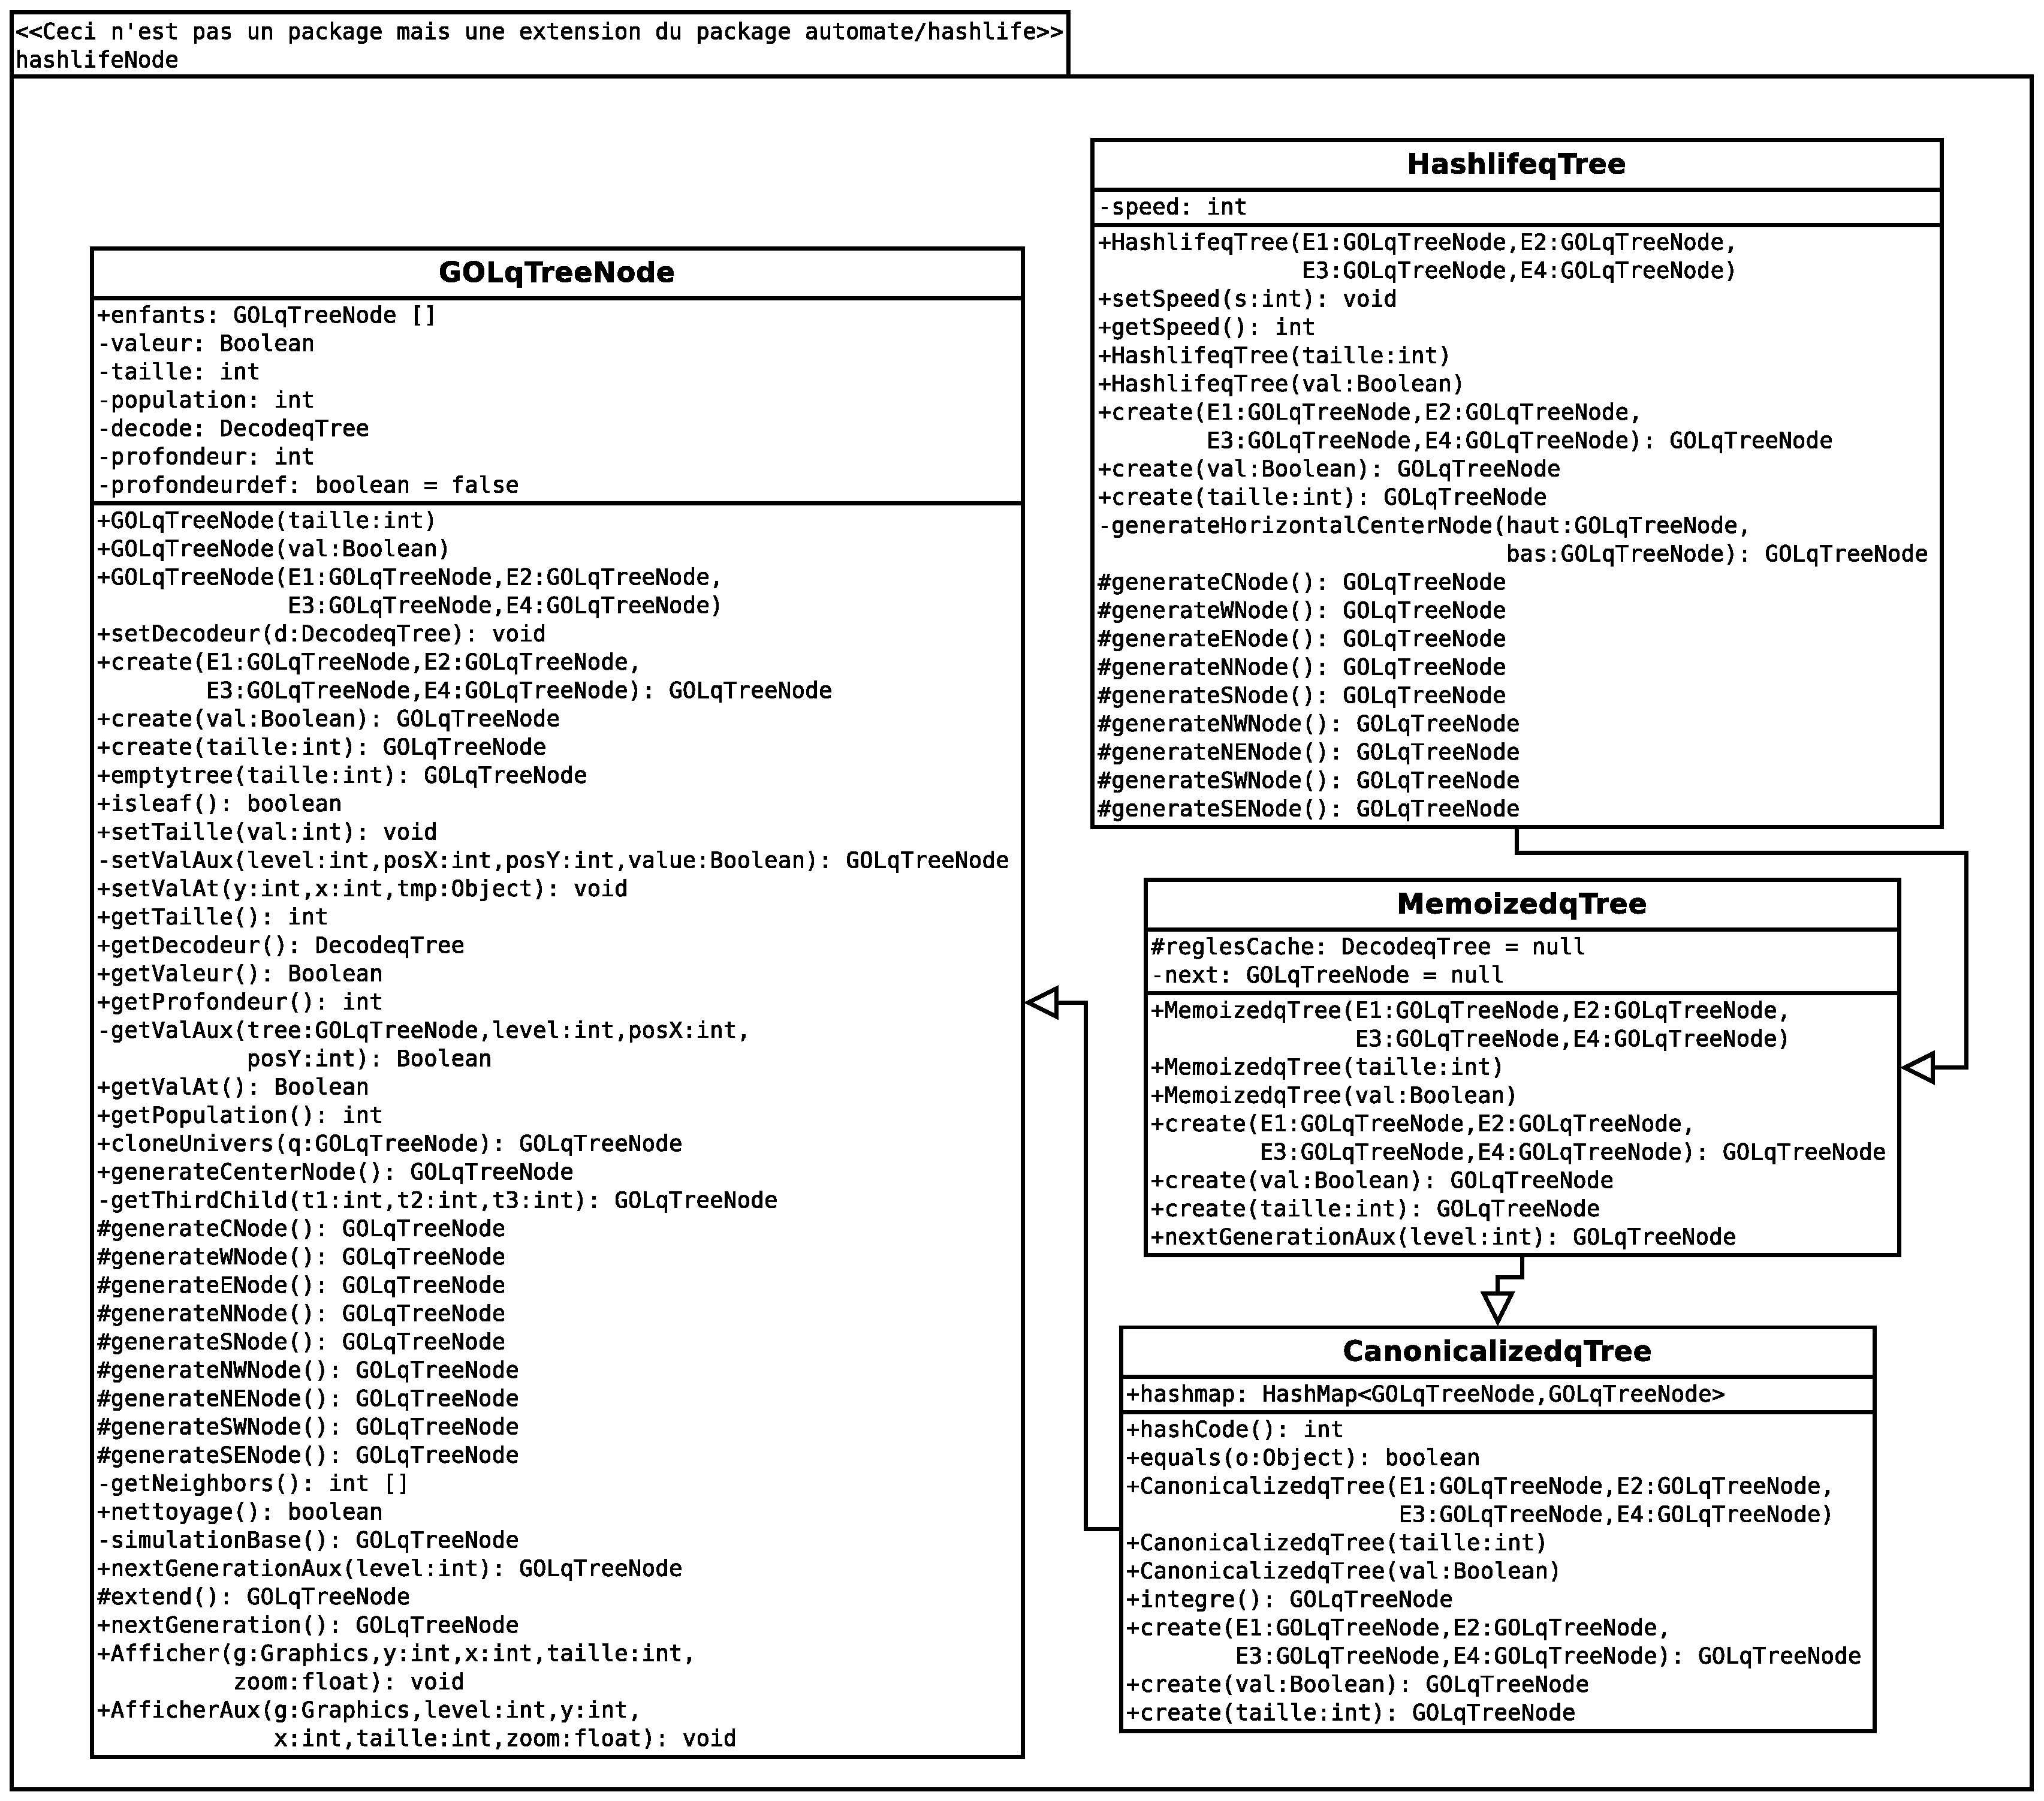
\includegraphics[scale=0.22]{images/Diagramme/package_automate_hashlifeNode.eps}
\caption{\label{fig:Automate/hashlifeNode}Illustration de la partie hashlifeNode du diagramme précédent}
\end{figure}
\subsection{Package Graphique}
\par Le package graphique regroupe tout ce qui a un rapport avec l'interface comme les interaction entre le clavier et l'interface via la classe \textbf{Clavier} qui implémente l'interface KeyListener ou encore l'interface elle même (\textbf{InterfaceGameOfLife}) avec ces différents composants (\textbf{AffichagePrincipal}, \textbf{Menu}). 
\begin{figure}[htp]
\centering
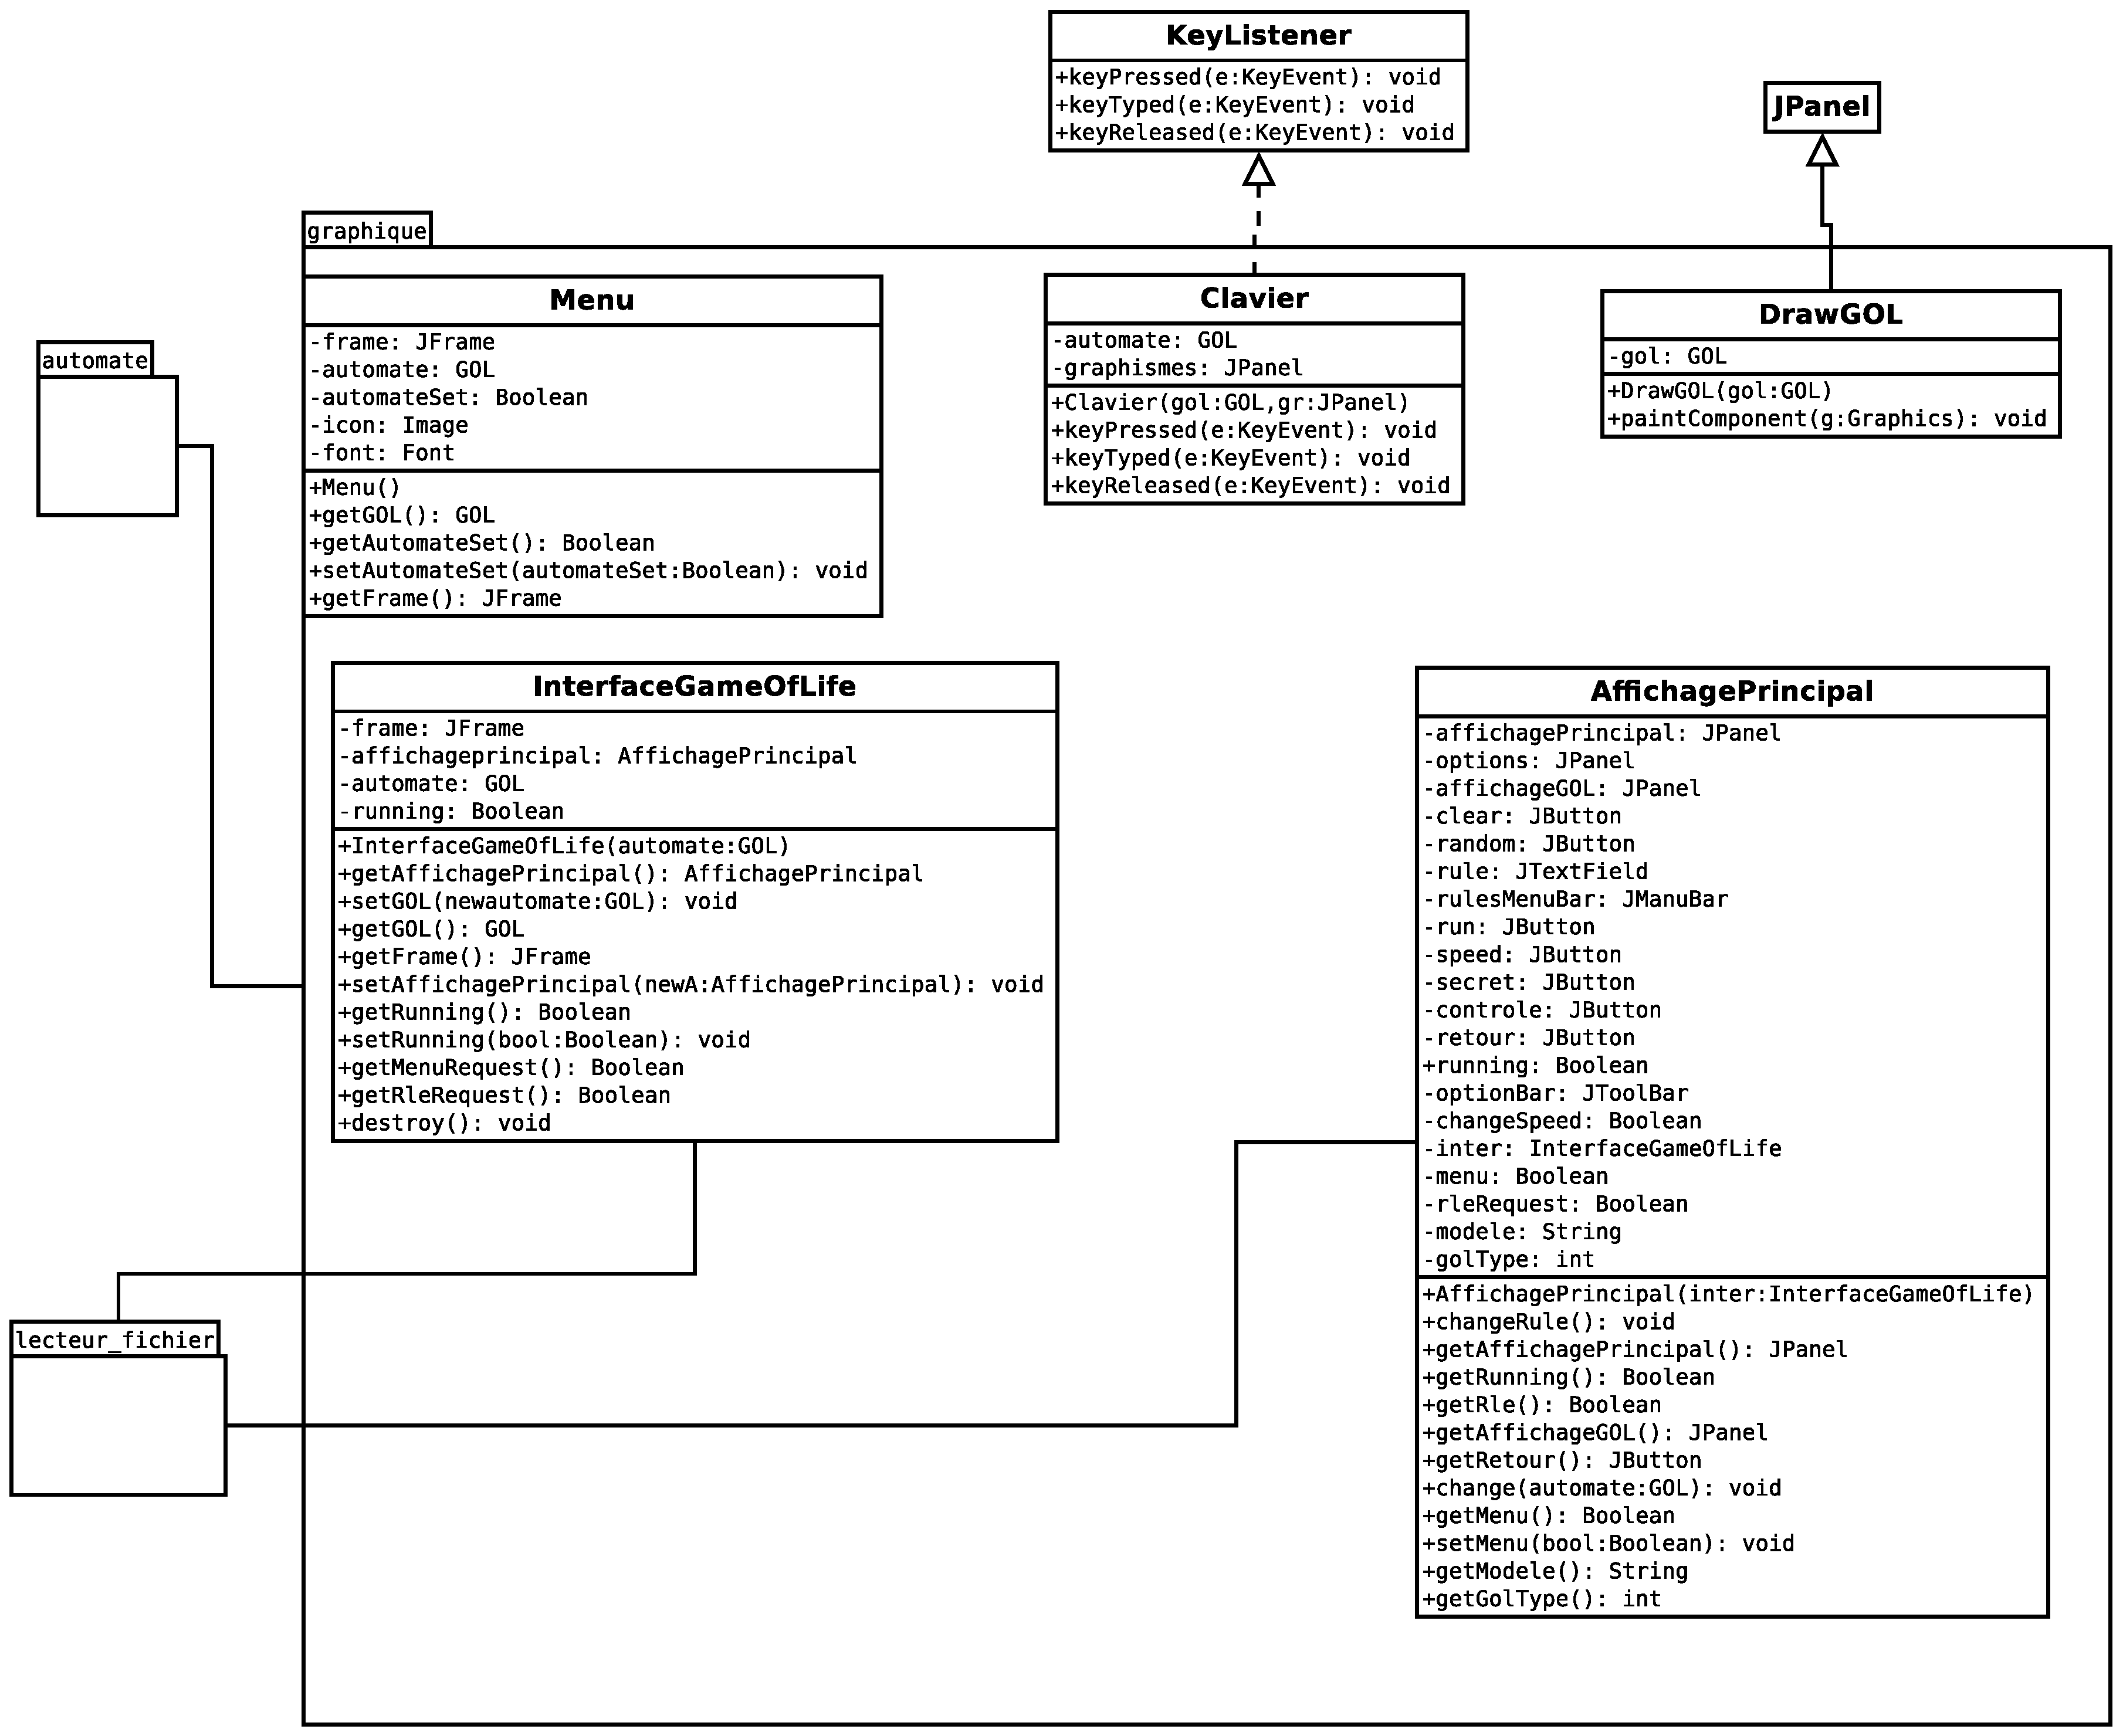
\includegraphics[scale=0.22]{images/Diagramme/package_graphique.eps}
\caption{\label{fig:Graphique}Illustration du package graphique}
\end{figure}
\subsection{Package Lecteur fichier}
\par Le package lecteur fichier contient les classes permettant la lecture des différents fichiers en ressources.\\
La classe \textbf{Lecture CSV} permet de lire un fichier CSV et renvoie les informations dans une liste de tableaux de chaînes de caractères (un tableau de chaînes de caractères représentent une ligne du fichier CSV). Cette classe a aussi d'autres méthodes permettant de rechercher le code (ou mode ou type d'univers aléatoire (uniquement pour les instance de \textbf{GOLGrilleLifeLike}))  du jeu de la vie ou de l'automate cellulaire grâce aux noms (ou au code) du jeu de la vie ou de l'automate cellulaire.\\
La classe \textbf{LecteurRLE} permet de charger un modèle RLE sur une instance de \textbf{GOL} après l'avoir récupéré et décodé de l'archive.
\\
Ce package va être réutilisé par les classes du package graphique ainsi que par le main.
\begin{figure}[htp]
\centering
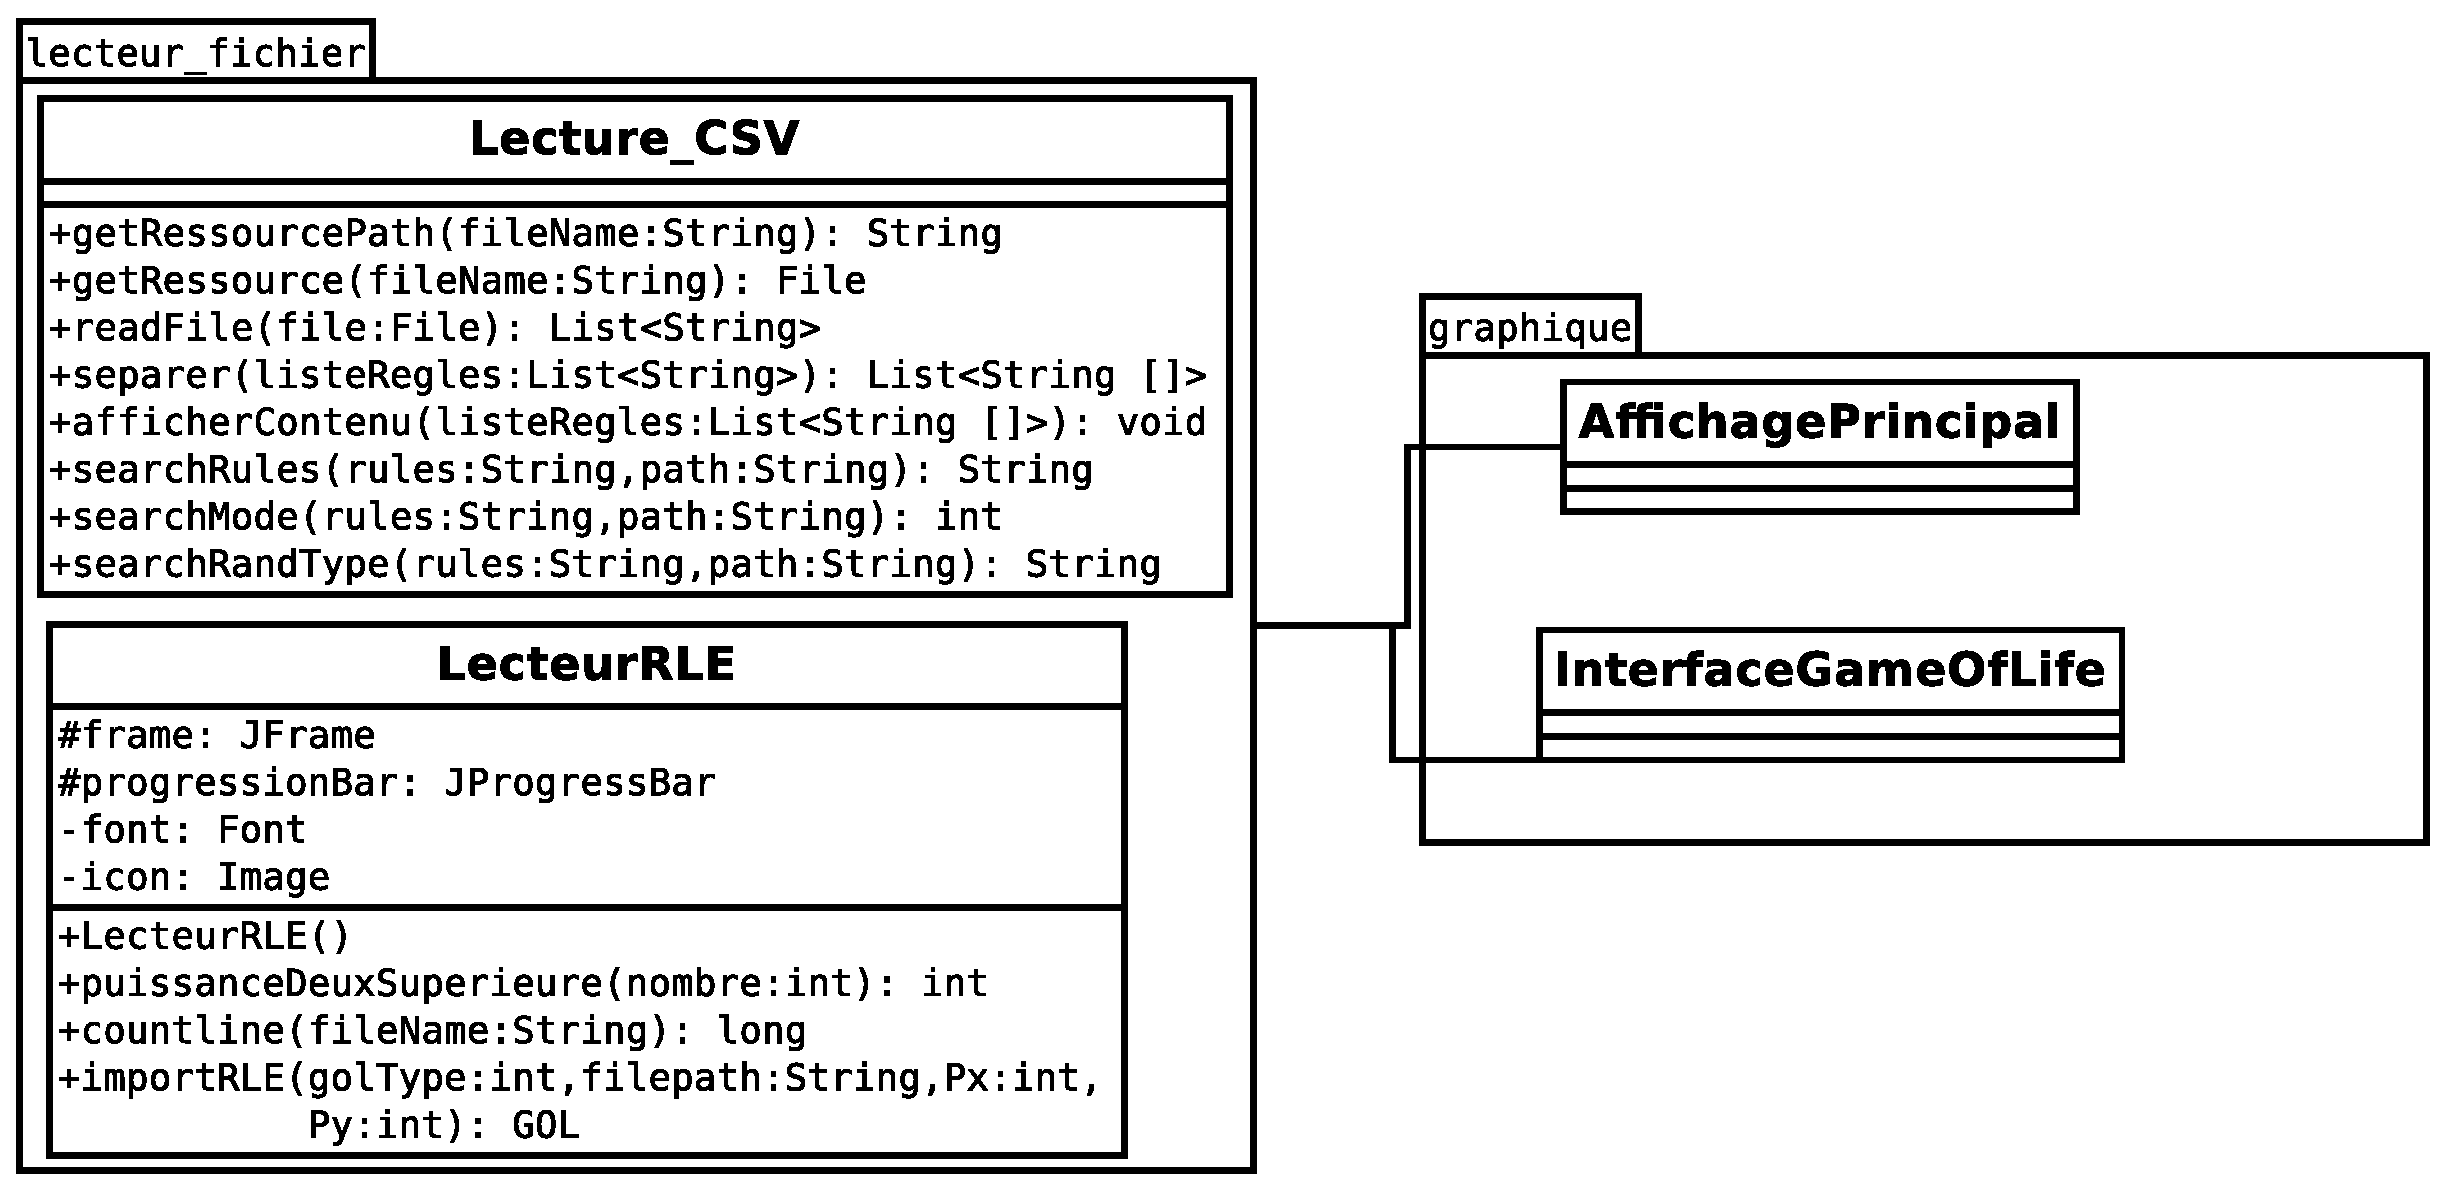
\includegraphics[scale=0.35]{images/Diagramme/package_lecteur_fichier.eps}
\caption{\label{fig:Lecteur_fichier}illustration du package lecteur fichier}
\end{figure}
\subsection{Package Test}
Ce package contient tout les test unitaires du projet permettant de savoir la validité des méthodes utilisées dans les différentes classes des package automate et lecteur fichier.

\end{document}
